\chapter{DASAR TEORI}
Pada bab ini akan dijelaskan mengenai dasar teori yang menjadi dasar pengerjaan Tugas Akhir ini.

\section{Deskripsi Permasalahan} \label{section:deskripsi_permasalahan}
Amr M. sangat curiga dengan sebuah iklan yang terdiri dari 2 buah \textit{string} $ad1$ dan $ad2$. Ia menduga kedua \textit{string} tersebut menyimpan pesan tersembunyi. Setelah menghubungi sumber yang terpercaya, ia menemukan proses untuk menyembunyikan pesan tersebut. Pesan asli yang dibawa selalu berupa dua buah \textit{string} $orig1$ dan $orig2$. Berikut adalah langkah-langkah transformasi pesan asli menjadi pesan pada iklan:

\begin{enumerate}
	\item Karakter-karakter pada \textit{string} $orig1$ diacak urutannya.
	\item Karakter-karakter pada \textit{string} $orig2$ diacak urutannya.
	\item Salah satu karakter dari \textit{string} $orig1$ atau $orig2$ diganti dengan karakter sebelum atau sesudahnya dalam alfabet.
\end{enumerate}

Langkah-langkah di atas akan menghasilkan \textit{string} $ad1$ dan $ad2$ dari $orig1$ dan $orig2$ secara berurutan. Contohnya untuk \textit{string} $orig1 = bcd $ dan $orig2 = wcy$ dapat menghasilkan \textit{string} $ad1 = dcb$ dan $ad2 = cxy$ di mana $cxy$ berasal dari $wcy$ yang diacak menjadi $cwy$ dan karakter $w$ digantikan dengan karakter $x$.

Setelah melakukan riset, Amr menemukan sebuah jarak $X$, di mana $X$ adalah $jarak(orig1 + ad1)$ ditambah dengan $jarak(orig2 + ad2)$. Jarak antara dua \textit{string} didefinisikan sebagai jumlah dari selisih absolut dari karakter-karakter pada posisi yang sama. Contohnya $jarak(ab, cd) = |'a' - 'c'| + |'b' - 'd'| = 4$. Diberikan \textit{string} $ad1$, $ad2$ dan sebuah bilangan bulat $X$. Hitung jumlah kemungkinan \textit{string} $orig1$ dan $orig2$ yang mungkin.

Sebagai contoh, Tabel \ref{tab:contoh_kombinasi_c_n_1} adalah kombinasi dari \textit{string} $ orig1 $ dan $ orig2 $ dengan \textit{string} $ ad1=c $, \textit{string} $ ad2=n $ dan $ X=1 $. Jawaban dari kasus tersebut adalah 4 karena terdapat 4 kombinasi dengan $ X=1 $. Contoh berikutnya adalah kasus ketika $ ad1=bd $, \textit{string} $ ad2=gj $ dan $ X=5 $. Berdasarkan daftar kombinasi \textit{string} $ orig1 $ dan $ orig2 $ pada Tabel \ref{tab:contoh_kombinasi_bd_gj_5}, terdapat $ 8 $ kombinasi \textit{string} $ orig1 $ dan \textit{string} $ orig2 $ yang memenuhi kriteria $ X = 5 $ sehingga jawaban akhir dari kasus tersebut adalah $ 8 $. 

\begin{table}
	\centering
	\begin{tabular}{|>$l<$|>$l<$|>$l<$|l|} \hline
		$ orig1 $ & $ orig2 $ & $ X $ & Validitas\\ \hline
		$ b $ & $ n $ & $ 1 $ & Valid \\ \hline
		$ d $ & $ n $ & $ 1 $ & Valid\\ \hline
		$ c $ & $ m $ & $ 1 $ & Valid\\ \hline
		$ c $ & $ o $ & $ 1 $ & Valid\\ \hline
	\end{tabular}
	\caption{Kombinasi \textit{string} $orig1$ dan $ orig2 $ dengan $ ad1 = c $, \textit{string} $ ad2 = n $ dan $ X=1 $}
	\label{tab:contoh_kombinasi_c_n_1}
\end{table}

\begin{table}
	\centering
	\begin{tabular}{|>$l<$|>$l<$|>$l<$|l|} \hline
		$ orig1 $ & $ orig2 $ & $ X $ & Validitas\\ \hline
		$ad$ & $gj$ & $1$ & Tidak valid\\ \hline
		$cd$ & $gj$ & $1$ & Tidak valid\\ \hline
		$bc$ & $gj$ & $1$ & Tidak valid\\ \hline
		$be$ & $gj$ & $1$ & Tidak valid\\ \hline
		$bd$ & $fj$ & $1$ & Tidak valid\\ \hline
		$bd$ & $hj$ & $1$ & Tidak valid\\ \hline
		$bd$ & $gi$ & $1$ & Tidak valid\\ \hline
		$bd$ & $gk$ & $1$ & Tidak valid\\ \hline
		$ad$ & $jg$ & $7$ & Tidak valid\\ \hline
		$cd$ & $jg$ & $7$ & Tidak valid\\ \hline
		$bc$ & $jg$ & $7$ & Tidak valid\\ \hline
		$be$ & $jg$ & $7$ & Tidak valid\\ \hline
		$bd$ & $ig$ & $5$ & Valid\\ \hline
		$bd$ & $kg$ & $7$ & Tidak valid\\ \hline
		$bd$ & $jf$ & $7$ & Tidak valid\\ \hline
		$bd$ & $jh$ & $5$ & Valid\\ \hline
		$cb$ & $gj$ & $3$ & Tidak valid\\ \hline
		$eb$ & $gj$ & $5$ & Valid\\ \hline
		$da$ & $gj$ & $5$ & Valid\\ \hline
		$dc$ & $gj$ & $3$ & Tidak valid\\ \hline
		$db$ & $fj$ & $5$ & Valid\\ \hline
		$db$ & $hj$ & $5$ & Valid\\ \hline
		$db$ & $gi$ & $5$ & Valid\\ \hline
		$db$ & $gk$ & $5$ & Valid\\ \hline
		$cb$ & $jg$ & $9$ & Tidak valid\\ \hline
		$eb$ & $jg$ & $11$ & Tidak valid\\ \hline
		$da$ & $jg$ & $11$ & Tidak valid\\ \hline
		$dc$ & $jg$ & $9$ & Tidak valid\\ \hline
		$db$ & $ig$ & $9$ & Tidak valid\\ \hline
		$db$ & $kg$ & $11$ & Tidak valid\\ \hline
		$db$ & $jf$ & $11$ & Tidak valid\\ \hline
		$db$ & $jh$ & $9$ & Tidak valid\\ \hline
	\end{tabular}
	\caption{Kombinasi \textit{string} $orig1$ dan $ orig2 $ dengan $ ad1 = bd $, \textit{string} $ ad2 = gj $ dan $ X=5 $}
	\label{tab:contoh_kombinasi_bd_gj_5}
\end{table}

\section{Deskripsi Umum}
Pada subbab ini akan dijelaskan  mengenai deskripsi-deskripsi umum yang terdapat pada Tugas Akhir ini.

\subsection{\textit{String}}
\label{subsec:string}
Pada dunia ilmu komputer, \textit{string} didefinisikan sebagai sebuah rangkaian karakter. \textit{String} pada umumnya dipahami sebagai sebuah struktur data dan diimplementasi menggunakan struktur data \textit{array}\cite{string}.

\subsection{Rekurens}
\label{subsec:rekurens}
Ketika sebuah algoritma mengandung sebuah persamaan rekursif yang memanggil dirinya sendiri, waktu prosesnya dapat dikatakan sebagai rekurens. Rekurens adalah sebuah persamaan atau pertidaksamaan yang mendeskripsikan sebuah fungsi dalam hal nilai pada masukan yang lebih kecil\cite{cormen}.

\subsection{\textit{Divide and Conquer}}
\label{subsec:divide_and_conquer}
Dalam ilmu komputer, \dc{} adalah paradigma perancangan algoritma yang bekerja dengan memecah permasalahan menjadi dua atau lebih submasalah dengan karakteristik yang sama atau berkaitan hingga cukup sederhana untuk diselesaikan secara langsung. Solusi dari masing-masing submasalah akan dikombinasikan untuk mendapatkan solusi dari permasalahan utama. Pada umumnya \dc{} merajuk pada aplikasi algoritma yang mereduksi setiap permasalahan menjadi hanya satu submasalah\cite{cp3}.

\subsection{\textit{Meet In The Middle}}
\label{subsec:meet_in_the_middle}
Dalam dunia pemrograman komputer, \textit{meet in the middle} adalah sebuah teknik pencarian dua arah dengan membagi dua permasalahan, lalu menyelesaikannya secara terpisah, lalu menggabungkan keduanya untuk mendapatkan hasil yang diinginkan\cite{cp3}.

\subsection{\textit{Dynamic Programming}}
\label{subsec:dynamic_programming}
Dalam dunia ilmu komputer, \dynamicprogramming{} adalah sebuah metode penyelesaian masalah yang memecah sebuah permasalahan yang rumit menjadi submasalah-submasalah yang lebih sederhana. \dynamicprogramming{} bersifat efektif ketika submasalah dari permasalahan yang diberikan mungkin berasal dari lebih dari satu pilihan. Teknik kunci dari \dynamicprogramming{} adalah menyimpan solusi untuk setiap submasalah untuk digunakan jika submasalah tersebut muncul kembali\cite{cormen}.

\subsection{\textit{State}}
\label{subsec:state}
\textit{State} atau \textit{state variable} adalah himpunan variabel parameter dari sebuah submasalah dari permasalahan yang diberikan\cite{state}.

\subsection{\textit{Bitmask}}
\label{subsec:bitmask}
Bitmask adalah sebuah bilangan bulat yang disimpan dan direpresentasikan sebagai himpunan dari nilai \textit{boolean}. Salah satu contoh pemanfaatan teknik \textit{bitmasking} adalah penggunaan \textit{bitmask} sebagai salah satu index pada tabel memo pada teknik \dynamicprogramming{}\cite{cp3}.

\section{Analisa Submasalah Optimal}
\label{sec: analisa_submasalah_optimal}
Pada subbab ini akan dijelaskan mengenai submasalah-submasalah yang jawabannya dapat membangun jawaban akhir. Tujuan utama dari permasalahan yang diberikan adalah untuk mencari jumlah kemungkinan \textit{string} $orig1$ dan $orig2$ dari \textit{string} $ad1$ dan $ad2$ yang memiliki jarak $dist(orig1, ad1) + dist(orig2, ad2) = X$ yang berikutnya disebut dengan jawaban akhir. 

\subsection{Membagi Permasalah Menjadi Submasalah yang \textit{Independent}} \label{subsec:membagi_permasalahan_menjadi_dua_submasalah_yang_independent}

Pada \problem{}, jawaban akhir merupakan banyak kombinasi \textit{string} $ orig1 $ dan \textit{string} $ orig2 $ yang mungkin. Dapat dilihat bahwa perhitungan jumlah kombinasi \textit{string} $ orig1 $ dari \textit{string} $ ad1 $ dan perhitungan jumlah kombinasi \textit{string} $ orig2 $ dari \textit{string} $ ad2 $ tidak memiliki keterkaitan satu sama lain. Artinya adalah dapat dihitung jumlah kombinasi \textit{string} $ orig1 $ dari \textit{string} $ ad1 $ tanpa mempedulikan kondisi \textit{string} $ orig2 $. Begitu juga sebaliknya pada perhitungan jumlah kombinasi \textit{string} $ orig2 $. Dengan kata lain perhitungan jumlah kombinasi \textit{string} $ orig1 $ dan $ orig2 $ dapat dilakukan secara terpisah. Teknik tersebut disebut dengan \meetinthemiddle{}.

Apabila operasi \textit{replace} pada \problem{} diabaikan, maka jawaban akhir dari dapat dihitung dengan alur secara umum pada Gambar \ref{figure:ilustrasi_umum_penyelesaian_meet_in_the_middle_tanpa_operasi_replace}. Karena operasi \textit{replace} diabaikan, maka jawaban akhir dapat dibentuk dengan mencari seluruh kemungkinan pasangan \textit{string} $ orig1 $ yang memiliki jarak $ D $ terhadap \textit{string} $ ad1 $ dengan \textit{string} $ orig2 $ yang memiliki jarak $ X - D $ terhadap \textit{string} $ ad2 $. 

\begin{figure}
	\centerline{ 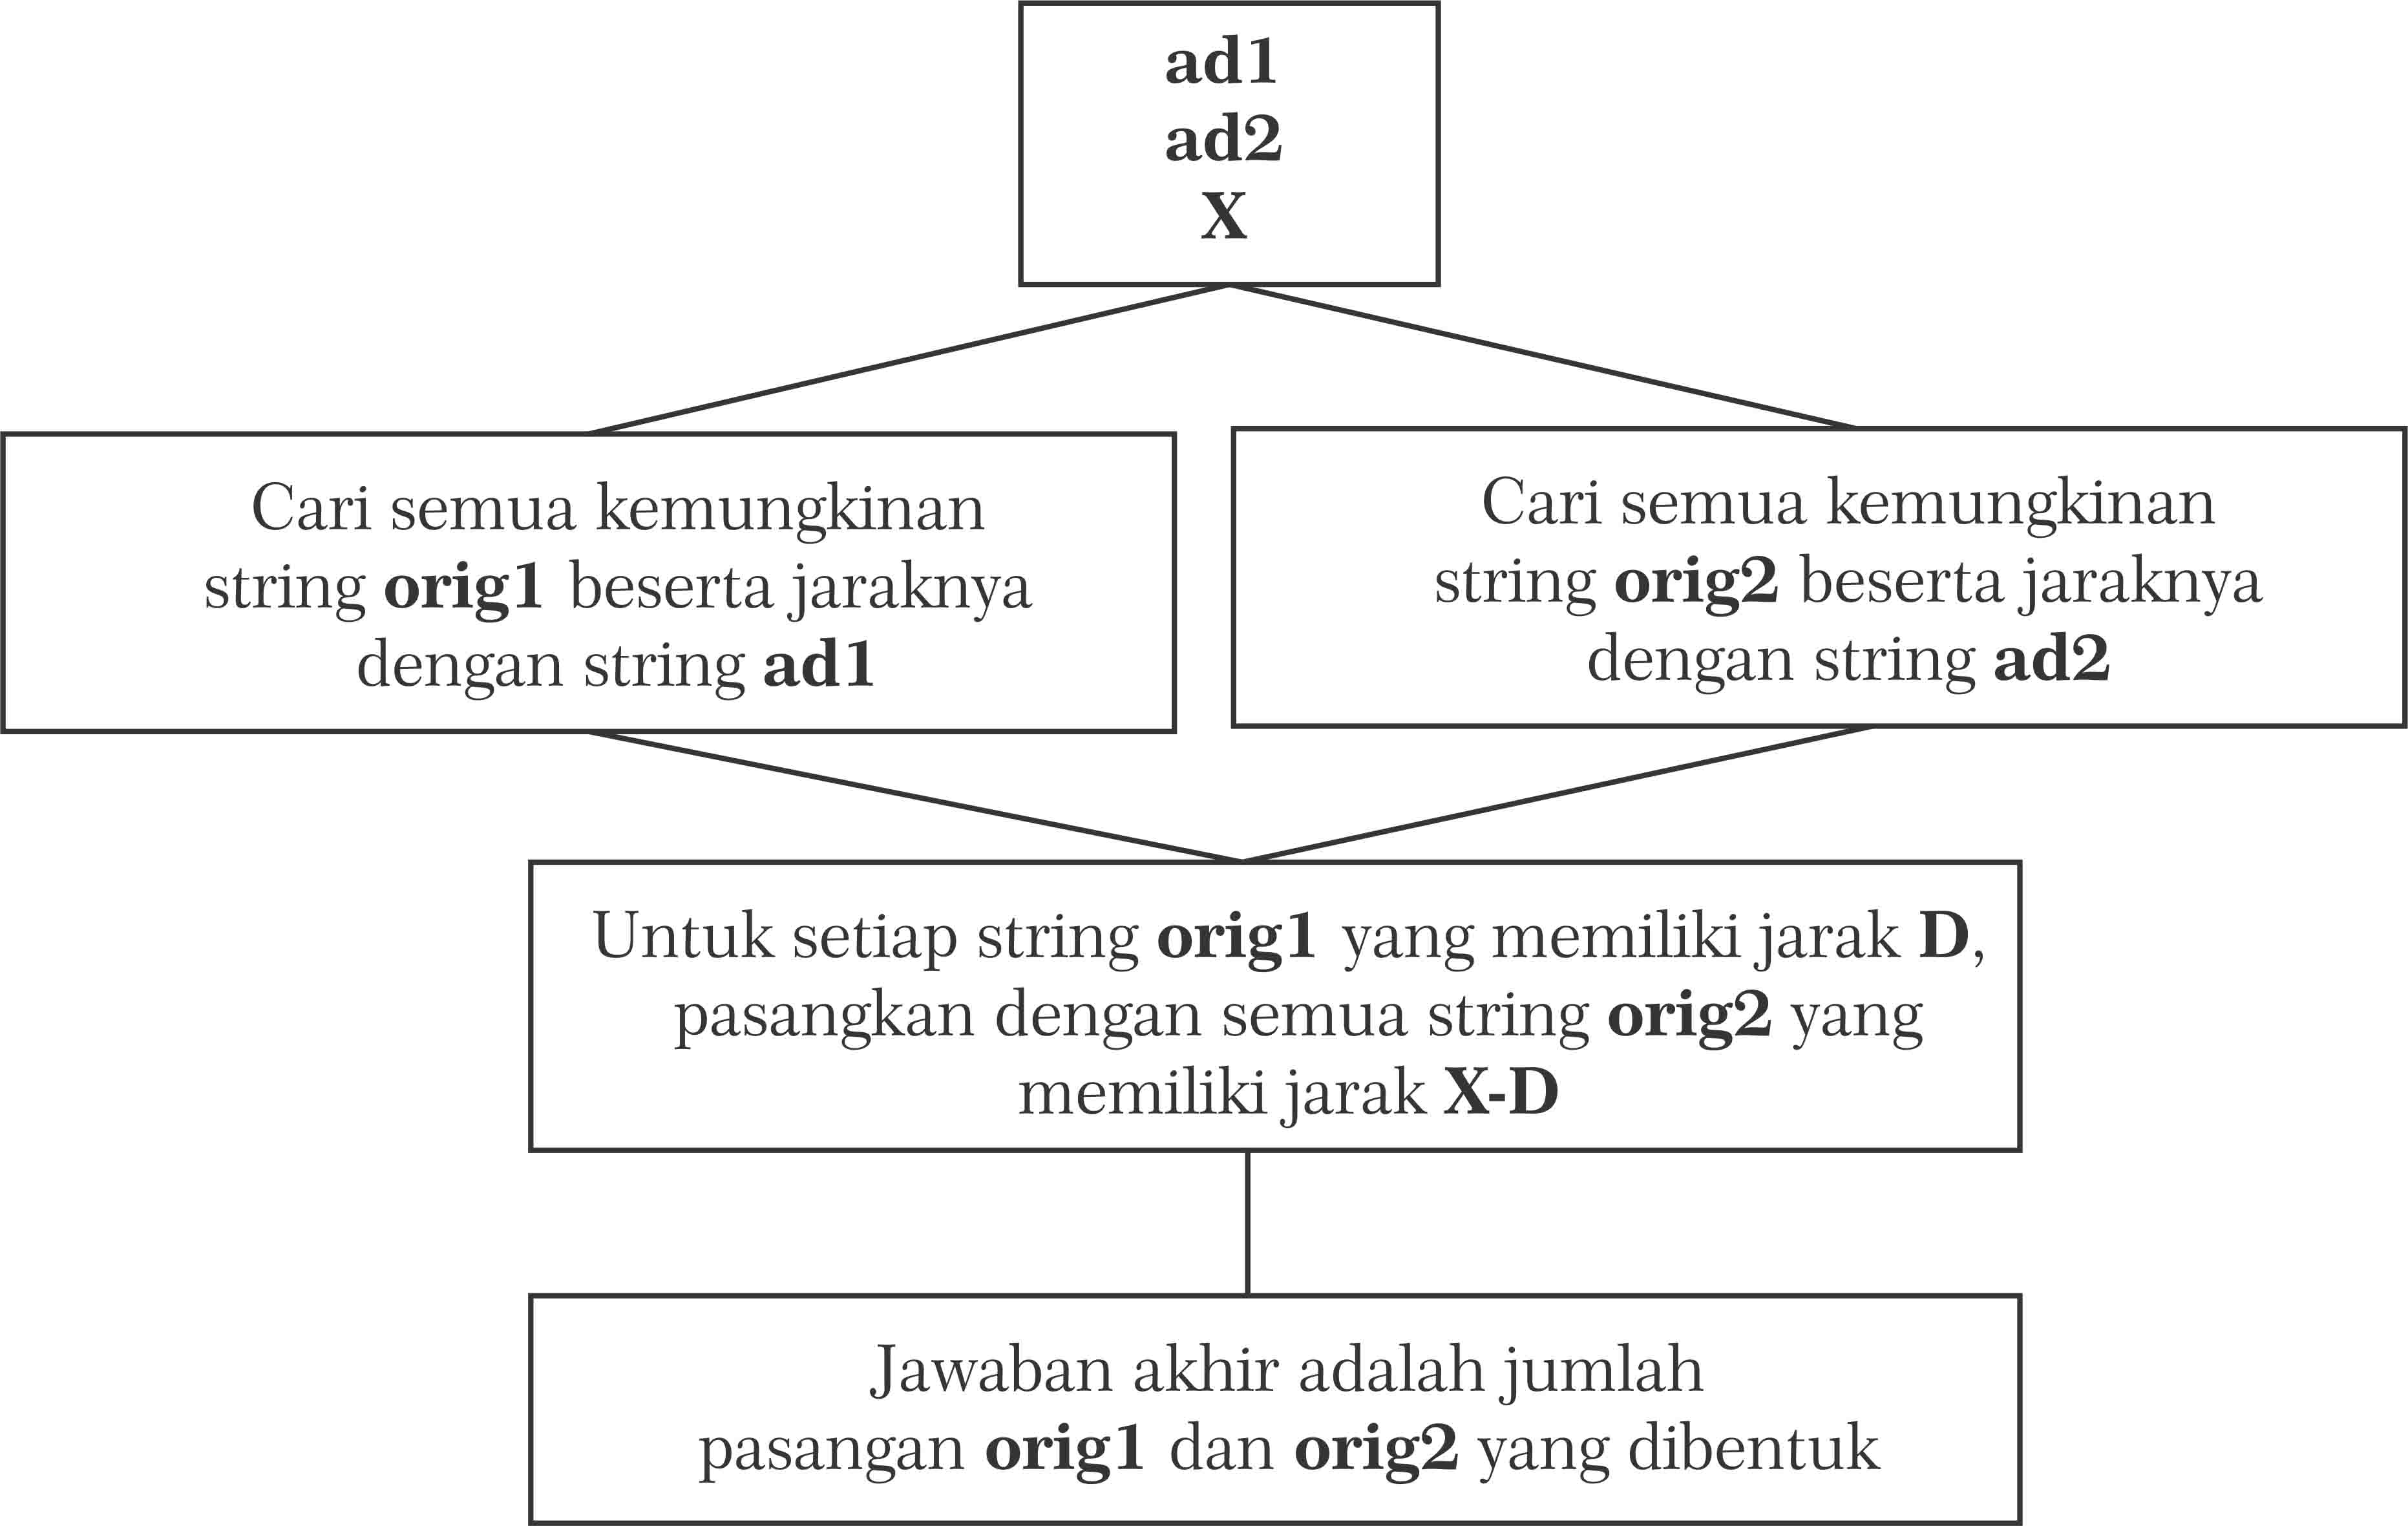
\includegraphics[scale=0.4]{assets/images/jpg/ilustrasi-umum-tanpa-replace.jpg}}
	\caption{Ilustrasi umum penyelesaian permasalahan dengan metode \meetinthemiddle{} tanpa operasi \textit{replace}}
	\label{figure:ilustrasi_umum_penyelesaian_meet_in_the_middle_tanpa_operasi_replace}
\end{figure}

Ketika terdapat operasi \textit{replace}, di mana operasi \textit{replace} adalah operasi di mana salah satu karakter pada \textit{string} $ orig1 $ atau $ orig2 $ diganti dengan karakter sebelumnya atau sesudahnya secara alfabetis, maka perlu dilakukan penyesuaian pada proses perhitungan jawaban. Selain perhitungan kombinasi \textit{string} $ orig1 $ dan \textit{string} $ orig2 $, perlu juga dilakukan perhitungan untuk kombinasi \textit{string} $ orig1 $ dan \textit{string} $ orig2 $ setelah dilakukan satu kali operasi \textit{replace}. Sehingga jawaban akhir dari \problem{} adalah total dari jumlah kemungkinan pasangan \textit{string} $ orig1 $ tanpa operasi \textit{replace} yang memiliki jarak $ D $ terhadap \textit{string} $ ad1 $ dengan \textit{string} $ orig2 $ dengan operasi \textit{replace} yang memiliki jarak $ X - D $ terhadap \textit{string} $ ad2 $ dan jumlah kemungkinan pasangan \textit{string} $ orig1 $ dengan operasi \textit{replace} yang memiliki jarak $ D $ terhadap \textit{string} $ ad1 $ dengan \textit{string} $ orig2 $ tanpa operasi \textit{replace} yang memiliki jarak $ X - D $ terhadap \textit{string} $ ad2 $. Gambar \ref{figure:ilustrasi_umum_penyelesaian_meet_in_the_middle_dengan_operasi_replace} adalah ilustrasi umum penyelesaian \problem{} dengan metode \meetinthemiddle{}.

\begin{figure}
	\centerline{ 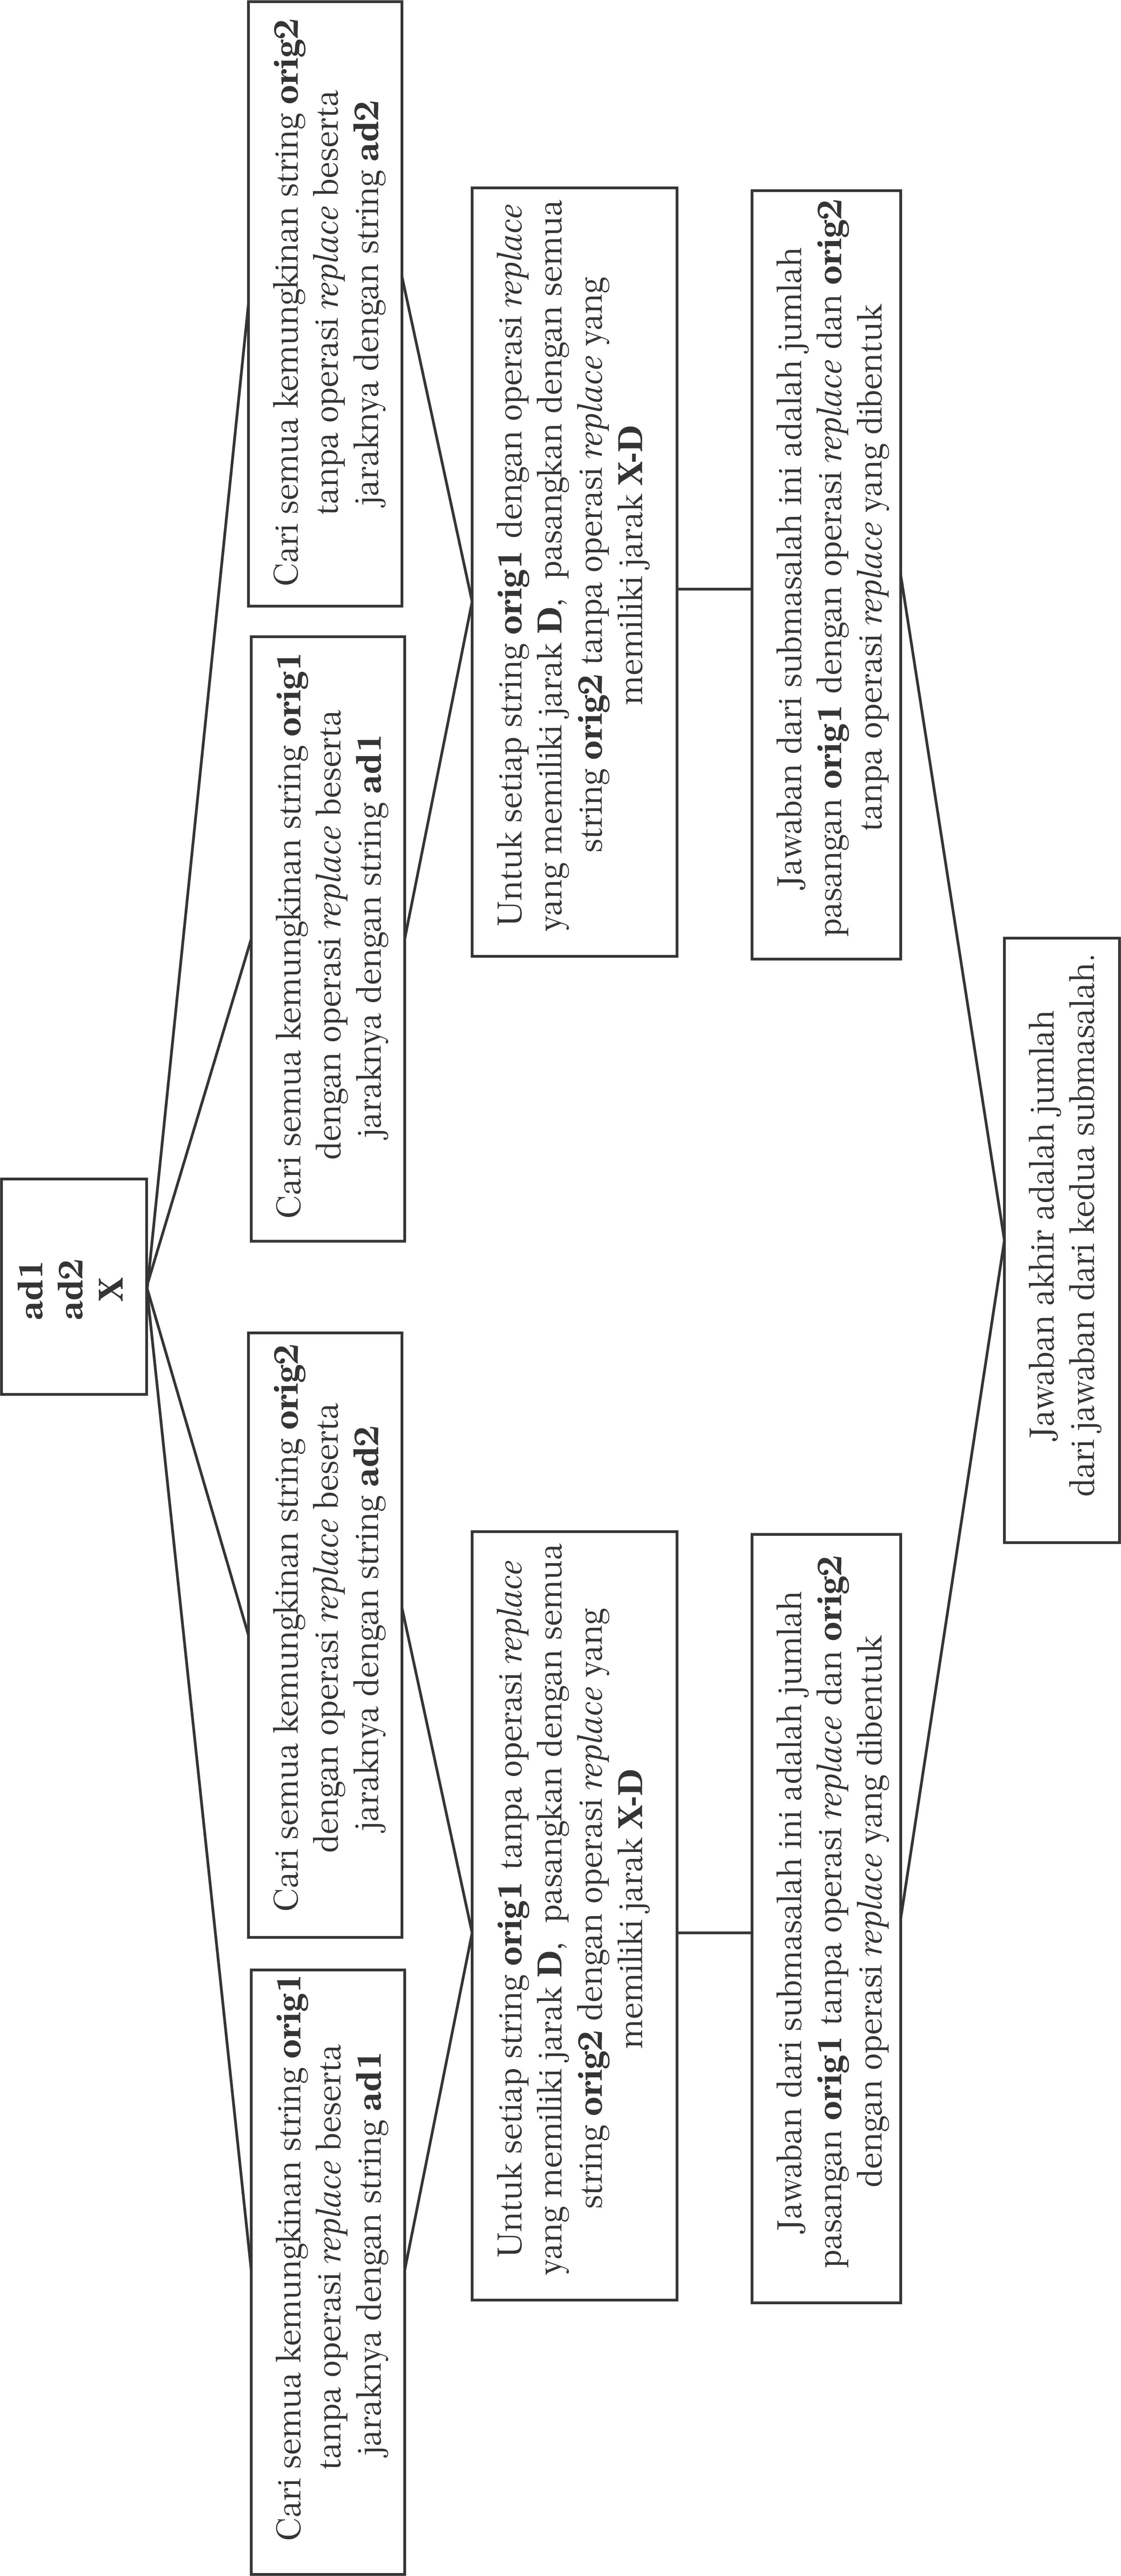
\includegraphics[scale=0.25]{assets/images/jpg/ilustrasi-umum-dengan-replace-rotated.jpg}}
	\caption{Ilustrasi umum penyelesaian permasalahan dengan metode \meetinthemiddle{} dengan operasi \textit{replace}}
	\label{figure:ilustrasi_umum_penyelesaian_meet_in_the_middle_dengan_operasi_replace}
\end{figure}

Sebagai contoh kasus ketika \textit{string} $ orig1=bd $, \textit{string} $ orig2=gj $ dan $ X=5 $. Langkah pertama untuk menyelesaikan kasus ini adalah dengan mencari semua kemungkinan kombinasi \textit{string} $ orig1 $ tanpa operasi \textit{replace} dan semua kemungkinan \textit{string} $ orig2 $ dengan operasi \textit{replace}. Tabel \ref{tab:kombinasi_orig1_bd_tanpa_replace} menunjukkan seluruh kombinasi \textit{string} $ orig1 $ tanpa operasi \textit{replace} beserta jarak masing-masing dengan \textit{string} $ ad1 $ dan Tabel \ref{tab:kombinasi_orig2_gj_dengan_replace} menunjukkan seluruh kombinasi \textit{string} $ orig2 $ dengan operasi \textit{replace} beserta jarak masing-masing dengan \textit{string} $ ad2 $. Berikutnya adalah mencari seluruh pasangan kombinasi \textit{string} $ orig1 $ tanpa operasi \textit{replace} dengan jarak terhadap \textit{string} $ ad1 $ sebesar $ D $ dan kombinasi \textit{string} $ orig2 $ dengan operasi \textit{replace} dengan jarak terhadap \textit{string} $ ad2 $ sebesar $ X-D $ yang hasilnya dapat dilihat pada Tabel \ref{tab:kombinasi_orig1_bd_tanpa_replace_dan_orig2_gj_dengan_replace}. Berikutnya hal yang sama juga dilakukan untuk kombinasi \textit{string} $ orig1 $ dengan operasi \textit{replace} dan \textit{string} $ orig2 $ tanpa operasi \textit{replace}. Tabel \ref{tab:kombinasi_orig1_bd_dengan_replace} menunjukkan seluruh kombinasi \textit{string} $ orig1 $ dengan operasi \textit{replace} beserta jarak masing-masing dengan \textit{string} $ ad1 $ dan Tabel \ref{tab:kombinasi_orig2_gj_tanpa_replace} menunjukkan seluruh kombinasi \textit{string} $ orig2 $ tanpa operasi \textit{replace} beserta jarak masing-masing dengan \textit{string} $ ad2 $. Berikutnya adalah mencari seluruh pasangan kombinasi \textit{string} $ orig1 $ dengan operasi \textit{replace} dengan jarak terhadap \textit{string} $ ad1 $ sebesar $ D $ dan kombinasi \textit{string} $ orig2 $ dengan operasi \textit{replace} tanpa jarak terhadap \textit{string} $ ad2 $ sebesar $ X-D $ yang hasilnya dapat dilihat pada Tabel \ref{tab:kombinasi_orig1_bd_dengan_replace_dan_orig2_gj_tanpa_replace}. Jawaban akhir dari kasus ketika \textit{string} $ orig1=bd $, \textit{string} $ orig2=gj $ dan $ X=5 $ adalah jumlah dari kombinasi pasangan \textit{string} $ orig1 $ dan \textit{string} $ orig2 $ pada Tabel \ref{tab:kombinasi_orig1_bd_tanpa_replace_dan_orig2_gj_dengan_replace} dan Tabel \ref{tab:kombinasi_orig1_bd_dengan_replace_dan_orig2_gj_tanpa_replace}.

\begin{table}
	\centering
	\begin{tabular}{|l|l|l|} \hline
		$ orig1 $ & Jarak dengan $ ad1 $\\ \hline
		$bd$ & $0$ \\ \hline
		$db$ & $4$ \\ \hline
	\end{tabular}
	\caption{Kombinasi \textit{string} $orig1$ dengan nilai \textit{string} $ ad1=bd $ tanpa operasi \textit{replace}}
	\label{tab:kombinasi_orig1_bd_tanpa_replace}
\end{table}

\begin{table}
	\centering
	\begin{tabular}{|l|l|l|} \hline
		$ orig2 $ & Jarak dengan $ ad2 $\\ \hline
		$fj$ & $1$ \\ \hline
		$hj$ & $1$ \\ \hline
		$gi$ & $1$ \\ \hline
		$gk$ & $1$ \\ \hline
		$ig$ & $5$ \\ \hline
		$kg$ & $7$ \\ \hline
		$jf$ & $7$ \\ \hline
		$jh$ & $5$ \\ \hline
	\end{tabular}
	\caption{Kombinasi \textit{string} $orig2$ dengan nilai \textit{string} $ ad2=gj $ dengan operasi \textit{replace}}
	\label{tab:kombinasi_orig2_gj_dengan_replace}
\end{table}

\begin{table}
	\centering
	\begin{tabular}{|l|l|l|l|} \hline
		$ orig1 $ & Jarak dengan $ ad1 $ & $ orig2 $ & Jarak dengan $ ad2 $\\ \hline
		$bd$ & $0$ & $ig$ & $5$\\ \hline
		$bd$ & $0$ & $jh$ & $5$\\ \hline
		$db$ & $4$ & $fj$ & $1$\\ \hline
		$db$ & $4$ & $hj$ & $1$\\ \hline
		$db$ & $4$ & $gi$ & $1$\\ \hline
		$db$ & $4$ & $gk$ & $1$\\ \hline
	\end{tabular}
	\caption{Kombinasi \textit{string} $orig1$ dengan nilai \textit{string} $ ad1=bd $ tanpa operasi \textit{replace} dan  \textit{string} $orig2$ dengan nilai \textit{string} $ ad2=gj $ dengan operasi \textit{replace} dengan $ X=5 $}
	\label{tab:kombinasi_orig1_bd_tanpa_replace_dan_orig2_gj_dengan_replace}
\end{table}

\begin{table}
	\centering
	\begin{tabular}{|l|l|l|} \hline
		$ orig1 $ & Jarak dengan $ ad1 $\\ \hline
		$ad$ & $1$ \\ \hline
		$cd$ & $1$ \\ \hline
		$bc$ & $1$ \\ \hline
		$be$ & $1$ \\ \hline
		$cb$ & $3$ \\ \hline
		$eb$ & $5$ \\ \hline
		$da$ & $5$ \\ \hline
		$dc$ & $3$ \\ \hline
	\end{tabular}
	\caption{Kombinasi \textit{string} $orig1$ dengan nilai \textit{string} $ ad1=bd $ dengan operasi \textit{replace}}
	\label{tab:kombinasi_orig1_bd_dengan_replace}
\end{table}

\begin{table}
	\centering
	\begin{tabular}{|l|l|l|} \hline
		$ orig2 $ & Jarak dengan $ ad2 $\\ \hline
		$gj$ & $0$ \\ \hline
		$jg$ & $6$ \\ \hline
	\end{tabular}
	\caption{Kombinasi \textit{string} $orig2$ dengan nilai \textit{string} $ ad2=gj $ tanpa operasi \textit{replace}}
	\label{tab:kombinasi_orig2_gj_tanpa_replace}
\end{table}

\begin{table}
	\centering
	\begin{tabular}{|l|l|l|l|} \hline
		$ orig1 $ & Jarak dengan $ ad1 $ & $ orig2 $ & Jarak dengan $ ad2 $\\ \hline
		$eb$ & $5$ & $gj$ & $0$\\ \hline
		$da$ & $5$ & $gj$ & $0$\\ \hline
	\end{tabular}
	\caption{Kombinasi \textit{string} $orig1$ dengan nilai \textit{string} $ ad1=bd $ dengan operasi \textit{replace} dan  \textit{string} $orig2$ dengan nilai \textit{string} $ ad2=gj $ tanpa operasi \textit{replace} dengan $ X=5 $}
	\label{tab:kombinasi_orig1_bd_dengan_replace_dan_orig2_gj_tanpa_replace}
\end{table}

Pada deskripsi \problem{} jawaban akhir adalah banyak kemungkinan \textit{string} $ orig1 $ dan $ orig2 $ tanpa perlu menyertakan daftar \textit{string} $ orig1 $ dan $ orig2 $ yang mungkin. Maka dari itu, proses perhitungan jawaban akhir dapat disederhanakan agar algoritma yang dibangun lebih optimal. Seperti yang terlihat pada ilustrasi umum penyelesaian pada Gambar \ref{figure:ilustrasi_umum_penyelesaian_meet_in_the_middle_dengan_operasi_replace_tanpa_kombinasi}, proses pencarian kombinasi \textit{string} $ orig1 $ dan $ orig2 $ dapat diganti dengan hanya menghitung jumlah kemungkinan kombinasi \textit{string} $ orig1 $ dengan atau tanpa operasi \textit{replace} dengan jarak terhadap \textit{string} $ ad1 $ sebesar $ D $ dan jumlah kemungkinan kombinasi \textit{string} $ orig2 $ dengan atau tanpa operasi \textit{replace} dengan jarak terhadap \textit{string} $ ad2 $ sebesar $ D $ dengan $ 0 \le D \le X $.

\begin{figure}
	\centerline{ 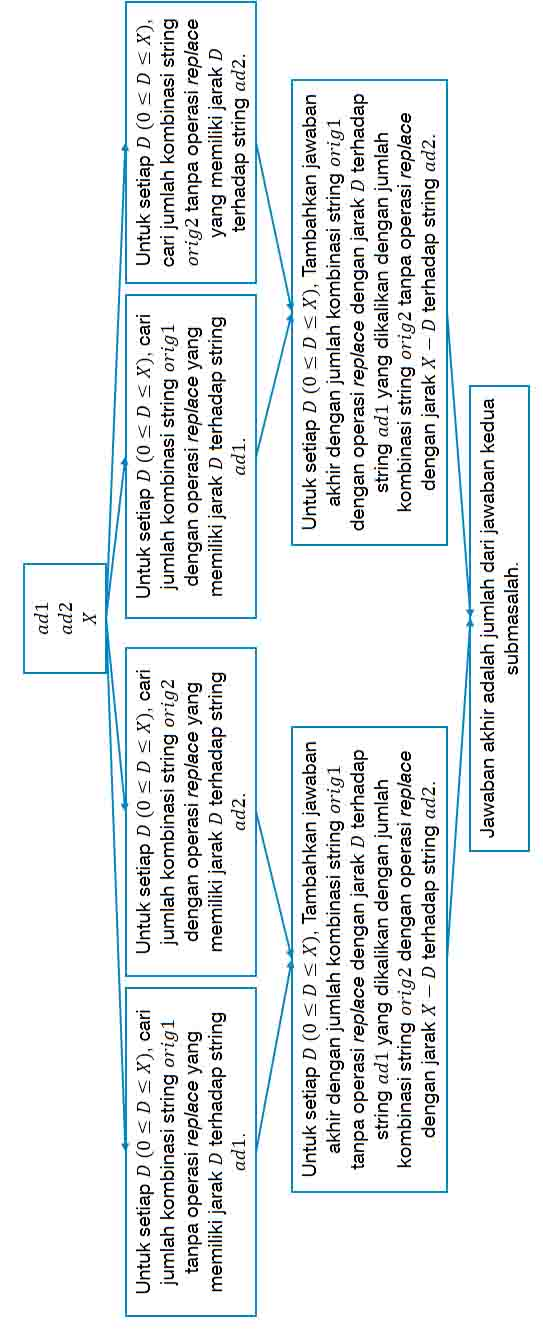
\includegraphics[scale=0.43]{assets/images/jpg/ilustrasi-umum-optimized-fix.jpg}}
	\caption{Ilustrasi umum penyelesaian permasalahan dengan metode \meetinthemiddle{} dengan operasi \textit{replace} tanpa mempedulikan kombinasi \textit{string} yang dihasilkan}
	\label{figure:ilustrasi_umum_penyelesaian_meet_in_the_middle_dengan_operasi_replace_tanpa_kombinasi}
\end{figure}

\subsection{Submasalah Optimal untuk Menghitung Jumlah Kombinasi \textit{String} $ Orig $ dari \textit{String} $ Ad $ Tanpa Operasi \textit{Replace} dengan Jarak $D$}
\label{subsec:submasalah_optimal_untuk_menghitung_jumlah_kombinasi_string_orig_dari_string_ad_tanpa_operasi_replace}
Ilustrasi pada Gambar \ref{figure:ilustrasi_umum_penyelesaian_meet_in_the_middle_dengan_operasi_replace_tanpa_kombinasi} menunjukkan bahwa untuk mendapatkan jawaban akhir dari \problem{} salah satu langkah yang harus dilakukan adalah menghitung jumlah kombinasi \textit{string} $ orig $ dari \textit{string} $ ad $ tanpa operasi \textit{replace} dengan jarak $ D $. Terdapat dua kali perhitungan untuk proses ini yaitu perhitungan untuk mencari jumlah kombinasi \textit{string} $ orig1 $ dan \textit{string} $ orig2 $ tanpa operasi \textit{replace} dengan jarak $ D $.

Perhitungan jumlah kombinasi \textit{string} $ orig $ tanpa operasi \textit{replace} dapat dilakukan dengan memanfaatkan teknik \textit{bitmasking}. Gambar \ref{figure:ilustrasi_perhitungan_kombinasi_orig_tanpa_replace} adalah ilustrasi perhitungan kombinasi \textit{string} $ orig $ dari \textit{string} $ ad $ dengan nilai \textit{string} $ ad=bcd $ dan $ D=4 $ tanpa operasi \textit{replace}. Nilai dari suatu \textit{state} adalah jumlah dari nilai seluruh \textit{state} yang merupakan \textit{child} dari \textit{state} tersebut dengan kasus dasar pada \textit{state} dengan $ mask=0 $, apabila $ jarak=D $ maka \textit{state} tersebut akan bernilai $ 1 $, jika tidak maka akan bernilai $ 0 $.

Namun, seperti yang dapat dilihat pada Gambar \ref{figure:contoh_kasus_tumpang_tindih}, terdapat beberapa kasus di mana pada suatu \textit{state}, \textit{state} dengan nilai tersebut bersifat tumpang tindih dengan suatu \textit{state} lain. Pada Gambar \ref{figure:contoh_kasus_tumpang_tindih}, \textit{state} yang saling tumpang tindih ditandai dengan tulisan berwarna merah. Dengan adanya kasus \textit{state} yang tumpang tindih tersebut dapat dimanfaatkan untuk melakukan optimasi pada algoritma yang dirancang dengan tidak melakukan perhitungan ulang pada \textit{state} yang sudah pernah muncul sebelumnya. Sehingga proses perhitungan yang sebelumnya seperti dengan ilustrasi pada Gambar \ref{figure:ilustrasi_perhitungan_kombinasi_orig_tanpa_replace} dapat disederhanakan menjadi seperti yang terdapat pada Gambar \ref{figure:ilustrasi_perhitungan_kombinasi_orig_tanpa_replace_optimal}. Teknik tersebut dikenal dengan teknik \dynamicprogramming{}.

\begin{figure}
	\centerline{ \includegraphics[scale=0.3]{assets/images/new/jpg/subproblem1-rotated.jpg}}
	\caption{Ilustrasi perhitungan jumlah kombinasi \textit{string} $ orig $ dari \textit{string} $ ad $ tanpa operasi \textit{replace} dengan nilai \textit{string} $ ad = bcd $ dan $ D=4 $}
	\label{figure:ilustrasi_perhitungan_kombinasi_orig_tanpa_replace}
\end{figure}

\begin{figure}
	\centerline{ \includegraphics[scale=0.3]{assets/images/new/jpg/subproblem1-overlapping-rotated.jpg}}
	\caption{Contoh kasus tumpang tindih pada perhitungan kombinasi \textit{string} $ orig $ dari \textit{string} $ ad $ tanpa operasi \textit{replace} dengan nilai \textit{string} $ ad=bcd $ dan $ D=4 $}
	\label{figure:contoh_kasus_tumpang_tindih}
\end{figure}

\begin{figure}
	\centerline{ 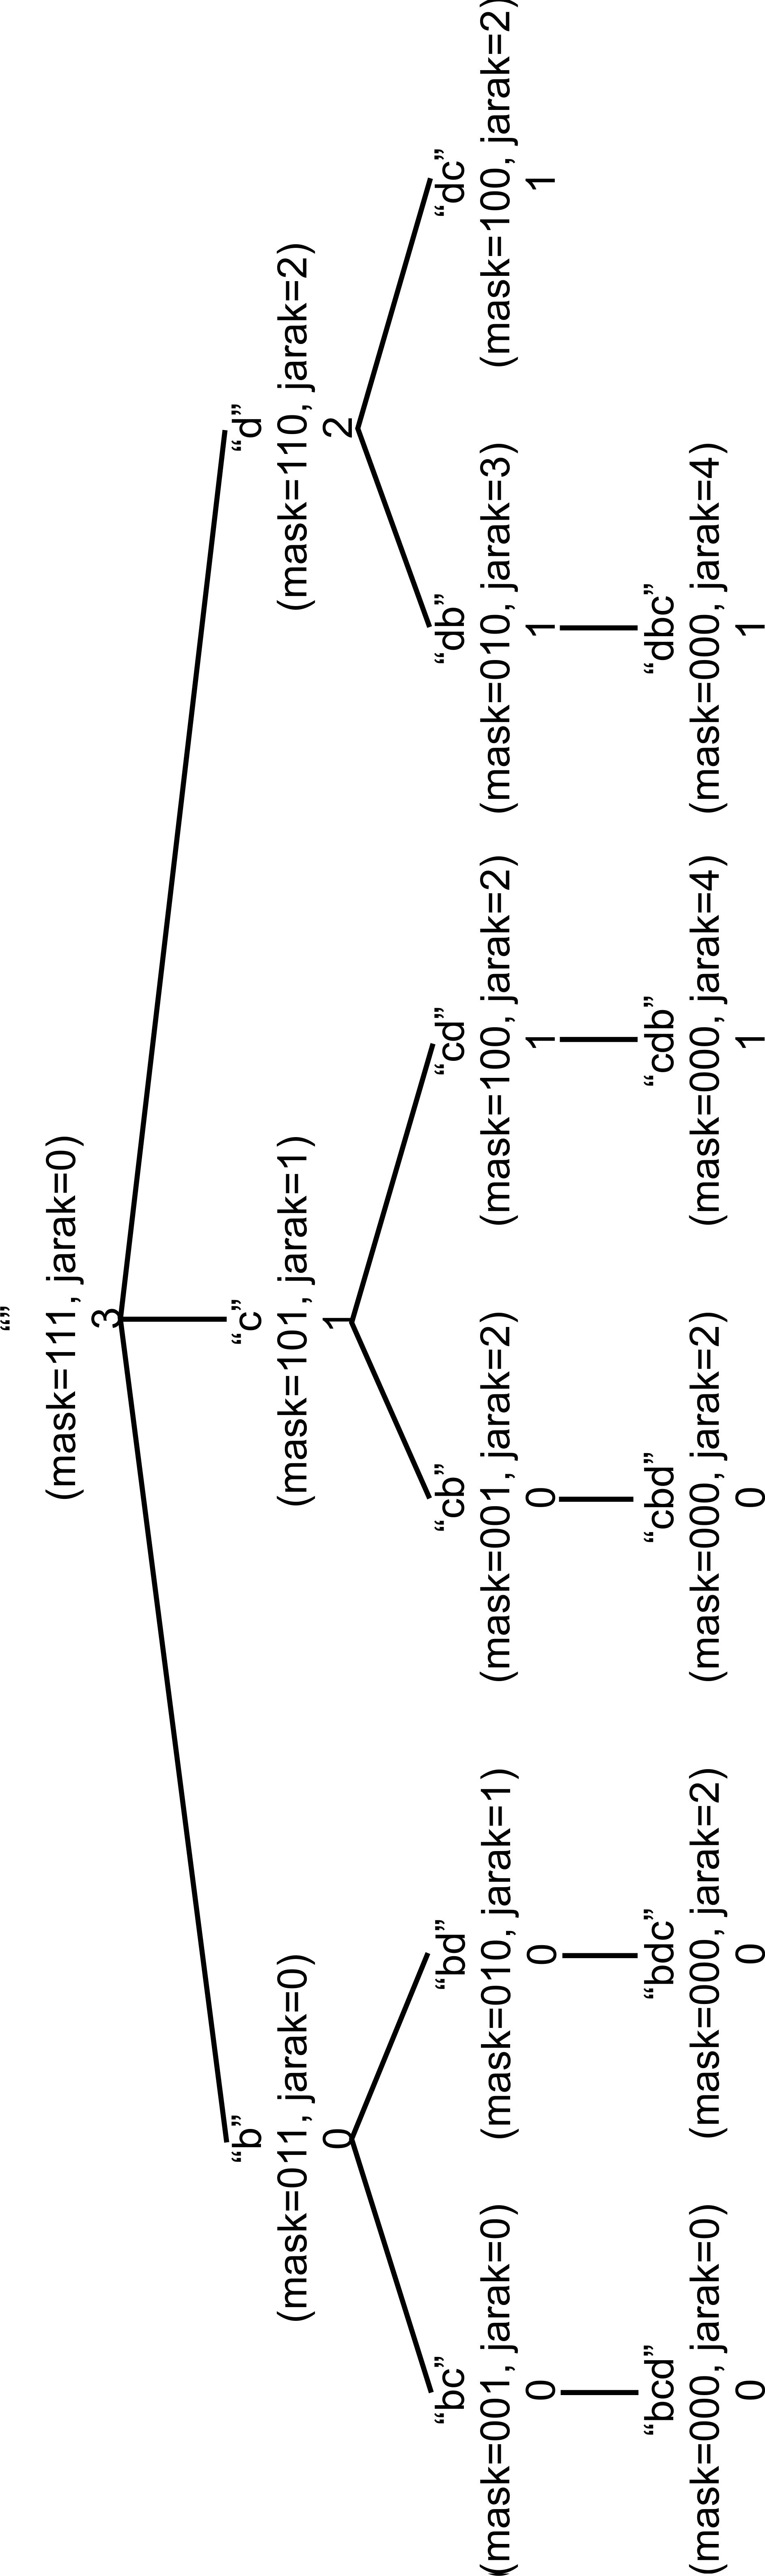
\includegraphics[scale=0.3]{assets/images/new/jpg/subproblem1-optimal-rotated.jpg}}
		\caption{Ilustrasi perhitungan jumlah kombinasi \textit{string} $ orig $ dari \textit{string} $ ad $ tanpa operasi \textit{replace} dengan nilai \textit{string} $ ad = bcd $ dan $ D=4 $ tanpa menghitung kasus yang tumpang tindih}
		\label{figure:ilustrasi_perhitungan_kombinasi_orig_tanpa_replace_optimal}
\end{figure}

\subsection{Submasalah Optimal untuk Menghitung Jumlah Kombinasi \textit{String} $ Orig $ dari \textit{String} $ Ad $ dengan Operasi \textit{Replace} dengan Jarak $D$}
\label{subsec:submasalah_optimal_untuk_menghitung_jumlah_kombinasi_string_orig_dari_string_ad_dengan_operasi_replace}

Ilustrasi pada Gambar \ref{figure:ilustrasi_umum_penyelesaian_meet_in_the_middle_dengan_operasi_replace_tanpa_kombinasi} menunjukkan bahwa untuk mendapatkan jawaban akhir dari \problem{} salah satu langkah yang harus dilakukan adalah menghitung jumlah kombinasi \textit{string} $ orig $ dari \textit{string} $ ad $ dengan operasi \textit{replace} dengan jarak $ D $. Terdapat dua kali perhitungan untuk proses ini yaitu perhitungan untuk mencari jumlah kombinasi \textit{string} $ orig1 $ dan \textit{string} $ orig2 $ tanpa operasi \textit{replace} dengan jarak $ D $.

Cara untuk mendapatkan jawaban dari submasalah ini hampir sama dengan cara mencari jawaban pada submasalah perhitungan jumlah kombinasi \textit{string} $ orig $ dari \textit{string} $ ad $ tanpa operasi \textit{replace}. Gambar \ref{figure:ilustrasi_perhitungan_kombinasi_orig_dengan_replace} merupakan ilustrasi dari penyelesaian submasalah perhitungan jumlah kombinasi \textit{string} $ orig $ dari \textit{string} $ ad $ dengan operasi \textit{replace} dengan nilai $ ad=be $ dan $ D=1 $. Sedikit berbeda dengan penyelesaian submasalah perhitungan jumlah kombinasi \textit{string} $ orig $ dari \textit{string} $ ad $ tanpa operasi \textit{replace}, pada penyelesaian submasalah ini terdapat satu parameter lagi pada setiap \textit{state}, yaitu penanda bahwa pada \textit{state} tersebut sudah pernah melakukan operasi \textit{replace} atau belum.

Sama seperti pada penyelesaian submasalah perhitungan jumlah kombinasi \textit{string} $ orig $ dari \textit{string} $ ad $ tanpa operasi \textit{replace}, pada submasalah perhitungan jumlah kombinasi \textit{string} $ orig $ dari \textit{string} $ ad $ dengan operasi \textit{replace} juga memiliki \textit{state} yang saling tumpang tindih seperti yang terlihat pada Gambar \ref{figure:contoh_kasus_tumpang_tindih_2} sehingga dapat dilakukan optimasi menggunakan teknik \dynamicprogramming{} untuk meningkatkan efisiensi algoritma yang dibangun. Pada Gambar \ref{figure:submasalah_1_pada_submasalah_2} dapat dilihat bahwa terdapat beberapa \textit{state} yang ternyata memiliki kondisi yang mampu diselesaikan dengan metode yang sama dengan metode penyelesaian submasalah perhitungan jumlah kombinasi \textit{string} $ orig $ dari \textit{string} $ ad $ tanpa operasi \textit{replace}. Sehingga penyelesaian submasalah perhitungan jumlah kombinasi \textit{string} $ orig $ dari \textit{string} $ ad $ dengan operasi \textit{replace} dapat disederhanakan dengan memanfaatkan penyelesaian submasalah perhitungan jumlah kombinasi \textit{string} $ orig $ dari \textit{string} $ ad $ tanpa operasi \textit{replace}.

\begin{figure}
	\centerline{ \includegraphics[scale=0.25]{assets/images/new/jpg/subproblem2-rotated.jpg}}
	\caption{Ilustrasi perhitungan jumlah kombinasi \textit{string} $ orig $ dari \textit{string} $ ad $ dengan operasi \textit{replace} dengan nilai \textit{string} $ ad = be $ dan $ D=1 $}
	\label{figure:ilustrasi_perhitungan_kombinasi_orig_dengan_replace}
\end{figure}

\begin{figure}
	\centerline{ 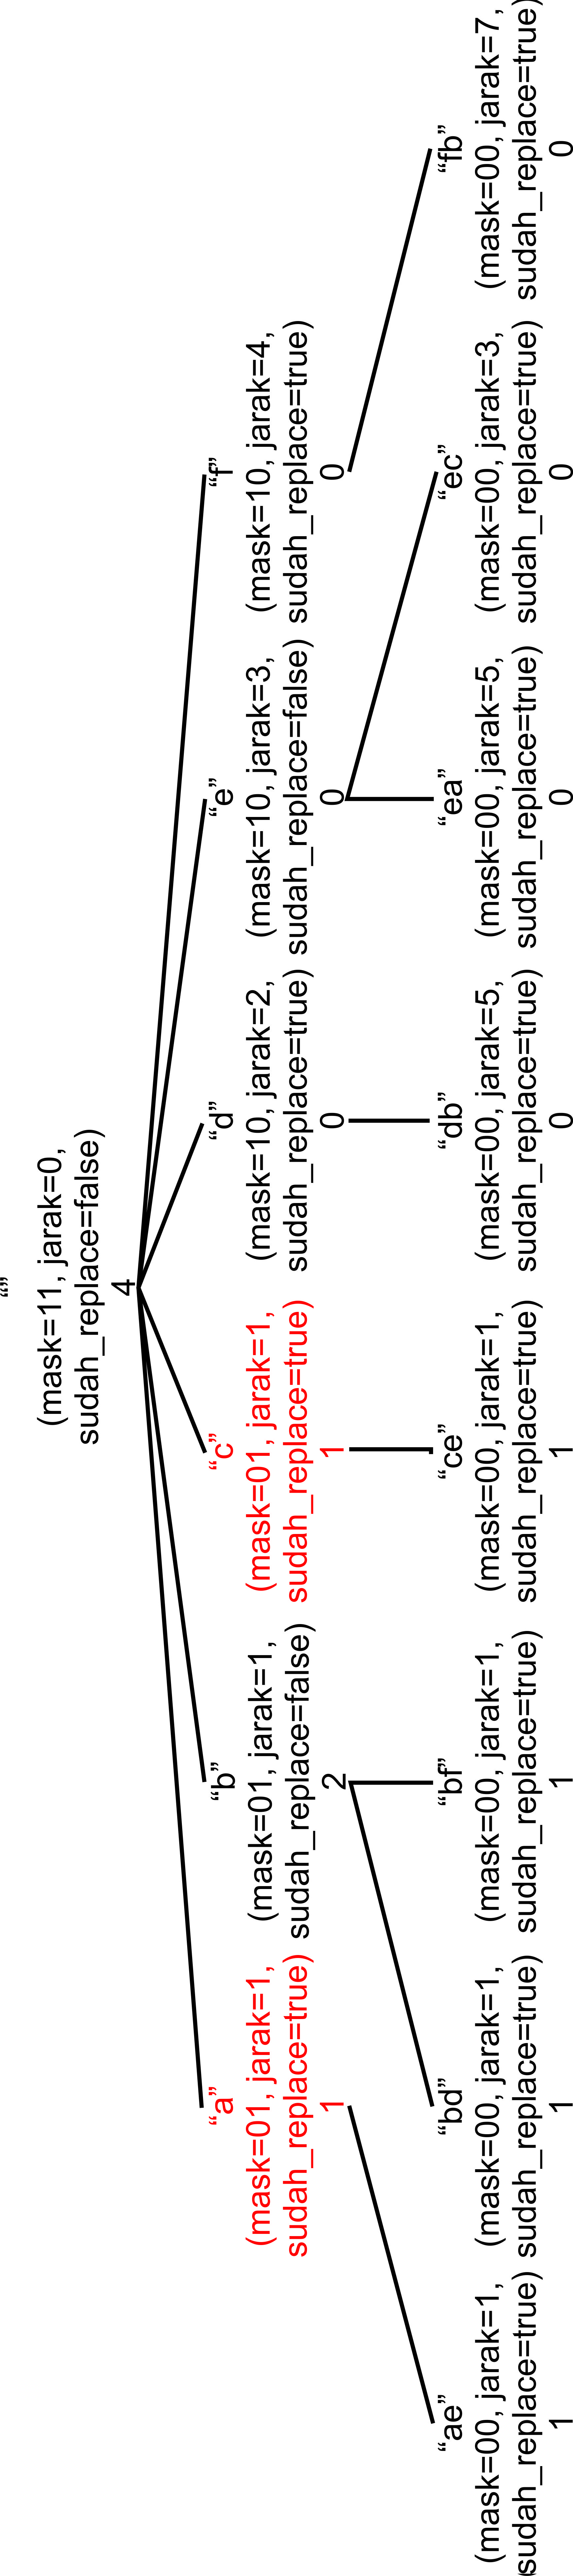
\includegraphics[scale=0.25]{assets/images/new/jpg/subproblem2-overlapping-rotated.jpg}}
	\caption{Contoh kasus tumpang tindih pada perhitungan kombinasi \textit{string} $ orig $ dari \textit{string} $ ad $ dengan operasi \textit{replace} dengan nilai \textit{string} $ ad=be $ dan $ D=1 $}
	\label{figure:contoh_kasus_tumpang_tindih_2}
\end{figure}

\begin{figure}
	\centerline{ 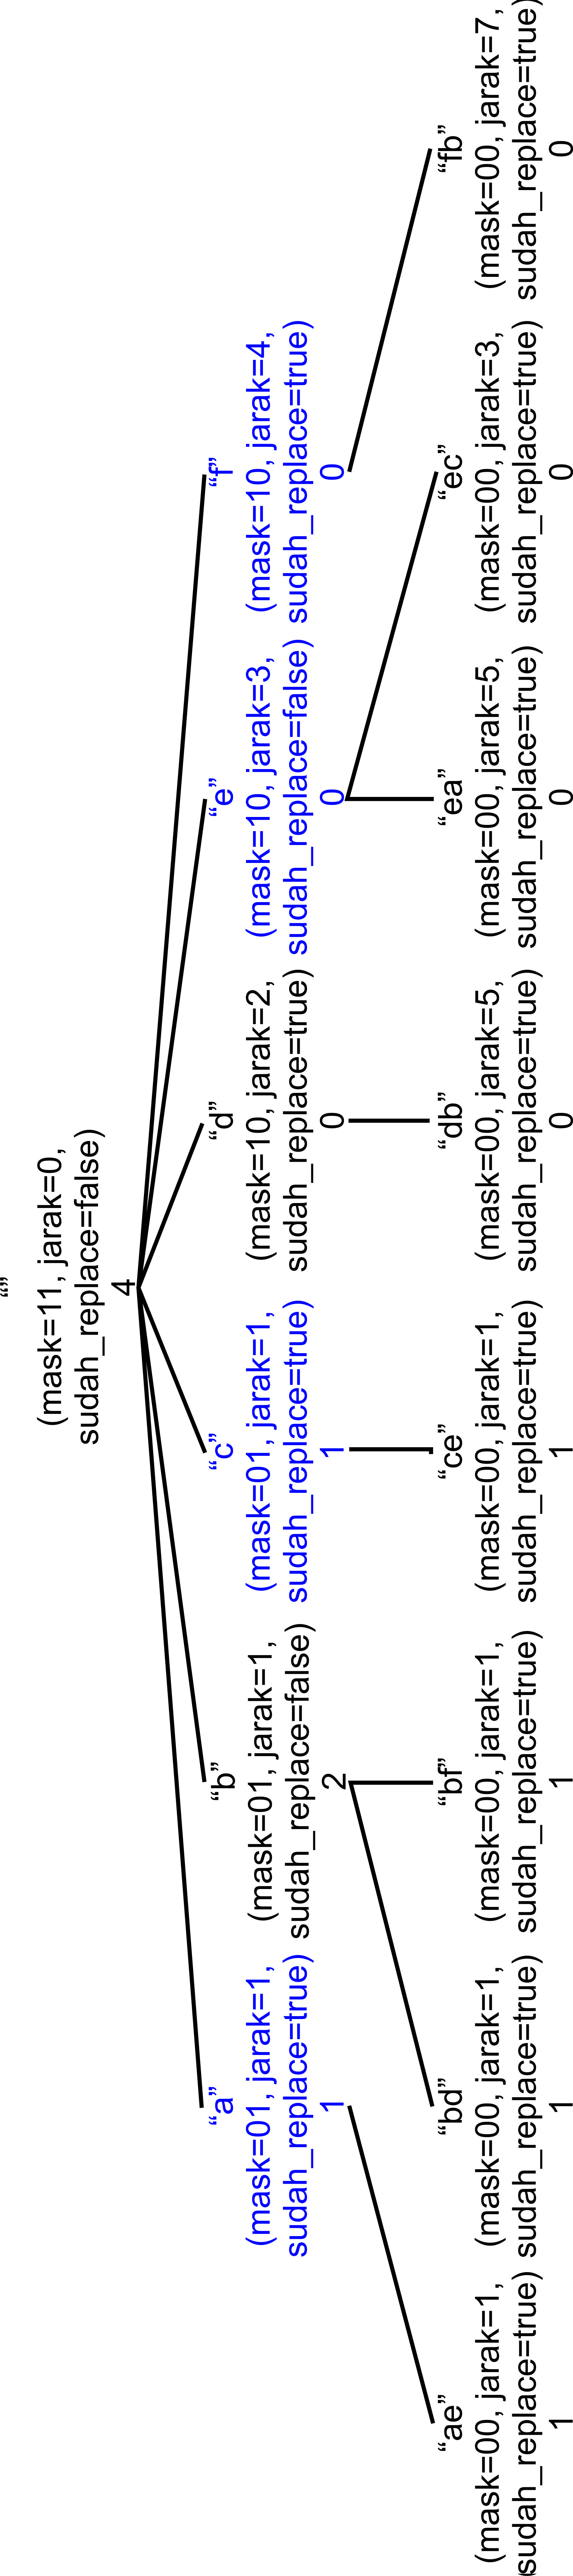
\includegraphics[scale=0.25]{assets/images/new/jpg/subproblem2-tipe1-rotated.jpg}}
	\caption{Submasalah perhitungan jumlah kombinasi \textit{string} $ orig $ terhadap \textit{string} $ ad $ tanpa operasi \textit{replace} pada submasalah perhitungan jumlah kombinasi \textit{string} $ orig $ terhadap \textit{string} $ ad $ dengan operasi \textit{replace}}
	\label{figure:submasalah_1_pada_submasalah_2}
\end{figure}


\section{Pemodelan Relasi Rekurens}
\label{sec:pemodelan_relasi_rekurens}
    
\begin{equation}
answer = \parbox[t]{0.9\textwidth}{ $\sum_{dist=0}^{dist=min_{(X, 250)}}((F_{(S_{0}, 2^{|S_{0}|}, bound - dist)} * G_{(S_{1}, 2^{|S_{1}|}, bound - X + dist)}) + (G_{(S_{0}, 2^{|S_{0}|}, bound -dist)} * F_{(S_{1},2^{|S_{1}|},bound-X+dist)}))$}
\label{equation:main_answer}
\end{equation}    
    
Pada subbab ini akan dijelaskan tentang relasi rekurens berdasarkan analisis pada subbab \ref{sec: analisa_submasalah_optimal}. Pada subbagian \ref{subsec:membagi_permasalahan_menjadi_dua_submasalah_yang_independent}, dijelaskan bahwa permasalahan dapat dipecah menjadi dua submasalah yang dapat diselesaikan tanpa bergantung satu sama lain dengan memecah permasalahan berdasarkan masing-masing \textit{string} $ad$. Karena terdapat sebuah operasi \textit{replace} yang dilakukan, maka untuk menyelesaikan masing-masing submasalah harus dilakukan dua jenis perhitungan, yaitu operasi perhitungan jumlah kemungkinan \textit{string} $orig$ tanpa operasi \textit{replace} dan operasi perhitungan jumlah kemungkinan \textit{string} $orig$ dengan operasi \textit{replace}. Kedua operasi tersebut didefinisikan dalam bentuk fungsi sebagai berikut:
\begin{enumerate}
	\item $F_{(S, mask, dist)}$, yaitu fungsi untuk menghitung jumlah kemungkinan \textit{string} awal dari \textit{string} $ S $ tanpa operasi \textit{replace} di mana $S$ adalah \textit{string} awal yang akan dihitung, $mask$ adalah nilai \textit{bitmask} dan $dist$ adalah jarak \textit{string} awal dengan \textit{string} yang dibentuk pada \textit{state} tersebut.
	\label{itm: fungsi_f}
	\item $G_{(S, mask, dist)}$, yaitu fungsi untuk menghitung jumlah kemungkinan \textit{string} awal dari \textit{string} $ S $ dengan sekali operasi \textit{replace} di mana $S$ adalah \textit{string} awal yang akan dihitung, $mask$ adalah nilai \textit{bitmask} dan $dist$ adalah jarak \textit{string} awal dengan \textit{string} yang dibentuk pada \textit{state} tersebut.
	\label{itm: fungsi_g} 
\end{enumerate}

Jawaban \problem{} dapat dihitung dengan memanfaatkan kedua fungsi di atas. Persamaan \ref{equation:main_answer} merupakan persamaan untuk menghitung jawaban utama dari \problem{} di mana $S_{0}$ adalah \textit{string} $ad1$, $S_{1}$ adalah \textit{string} $ad2$, $X$ adalah jumlah jarak($ad1$, $orig1$) dengan jarak($ad2$, $orig2$) dan $bound=min(250, X)$ dengan Tabel \ref{tab:daftar_notasi_main_answer} adalah daftar notasi yang digunakan pada persamaan tersebut. Nilai $ bound = min(250, X) $ memiliki arti batas atas variabel $ bound $ adalah $ 250 $ karena panjang \textit{string} masukan dijamin tidak lebih dari $ 10 $ karakter yang artinya jarak antar dua \textit{string} pada \problem{} tidak mungkin melebihi angka $ 250 $. Sehingga apabila nilai masukan $ X>250 $ dapat diasumsikan bahwa hal tersebut tidak mungkin. 

\begin{table}[H]
	\centering
	\begin{tabular} {|p{3cm}|p{5cm}|} \hline
		Notasi & Deskripsi\\ \hline
		$ dist $ & Nilai jarak yang diiterasi dari 0 hingga $ min(X, 250) $\\ \hline
		$ X $ & Masukan yang merepresentasikan jumlah jarak \textit{string} $ orig1 $ dengan \textit{string} $ ad1 $ dan jarak \textit{string} $ orig2 $ dengan \textit{string} $ ad2 $ \\ \hline
		$ S_{0} $ & \textit{String} masukan yang merepresentasikan $ ad1 $\\ \hline
		$ S_{1} $ & \textit{String} masukan yang merepresentasikan $ ad2 $\\ \hline
		$ |S_{0}| $ & Panjang \textit{string} $ ad1 $\\ \hline
		$ |S_{1}| $ & Panjang \textit{string} $ ad2 $\\ \hline
		$ bound $ & Nilai batas jarak maksimal yang bernilai $ min(X, 250) $\\ \hline
	\end{tabular}\caption{Daftar notasi persamaan \ref{equation:main_answer}}
	\label{tab:daftar_notasi_main_answer}
\end{table}

\subsection{Pemodelan Relasi Rekurens Submasalah Optimal untuk Menghitung Jumlah Kemungkinan \textit{String} Awal Tanpa Operasi \textit{Replace} dengan Jarak $X-dist$}
\label{subsec:pemodelan_relasi_rekurens_submasalah_optimal_untuk_menghitung_jumlah_kemungkinan_string_awal_tanpa_operasi_replace}

\begin{table}
	\centering
	\begin{tabular} {|p{3cm}|p{5cm}|} \hline
		Notasi & Deskripsi\\ \hline
		$ S $ & \textit{String} yang akan dicari kemungkinan \textit{string} awalnya.\\ \hline
		$ mask $ & Sebuah bilangan bulat yang bertugas sebagai \textit{bitmask} yang merepresentasikan kondisi karakter mana saja yang sudah diambil pada kondisi (\textit{state}) tersebut.\\ \hline
		$ dist $ & Jarak \textit{string} yang sudah terbentuk pada kondisi tersebut dengan \textit{string} $ S $ dari $ bound $ atau secara matematis dapat dituliskan dengan $ bound - distance(currentString, S) $.\\ \hline
		$ bound $ & Nilai batas jarak maksimal yang bernilai $ min(X, 250) $\\ \hline
		$ idx $ & Index karakter pada \textit{string} $ S $ yang akan diambil atau digunakan.\\ \hline
		$ NSB_{(mask)} $ & Mengembalikan jumlah angka 1 pada $ mask $ apabila direpresentasikan dalam basis biner\\ \hline
		$ set\_bit_{(mask)} $ & Himpunan index bilangan bernilai satu dari $ mask $ apabila direpresentasikan dalam basis biner.\\ \hline
		$ is\_on_{(mask, idx)} $ & Mengembalikan nilai $ true $ apabila bilangan pada index $ idx $ pada $ mask $ bernilai $ 1 $ apabila direpresentasikan dalam basis biner.\\ \hline
	\end{tabular}\caption{Daftar notasi persamaan \ref{equation:rekurens_f}, \ref{equation:rekurens_f1} dan \ref{equation:rekurens_duplicate_rule1}}
	\label{tab:daftar_notasi_f}
\end{table}

\begin{equation}
F_{(S, mask, dist)} = \begin{cases}
0, & \parbox[t]{.3\textwidth}{if $dist > bound$ or ($mask=0$ and $dist \neq bound$)}, \\
1, & \parbox[t]{.3\textwidth}{if $mask=0$ and $dist=bound$}, \\
\sum_{i=0}^{i=NSB_{(mask)}} \\F1_{(S, mask,
	set\_bit(mask)_{i}, dist)} ,& \text{otherwise}
\end{cases}
\label{equation:rekurens_f}
\end{equation}



\begin{equation}
F1_{(S, mask, idx, dist)} = 
\begin{cases}
F_{(S, mask - 2^{idx}, dist +}\\_{|S_{idx} - S_{curIdx}|)}
, & \parbox[t]{.3\textwidth}{idx = |S| - 1 or $duplicate\_rule1_{(S, mask, idx)} = True$}\\
0, & \text{otherwise}
\end{cases}
\label{equation:rekurens_f1}
\end{equation}


\begin{equation}
duplicate\_rule1_{(S, mask, idx)} = 
\begin{cases}
True, & \parbox[t]{.3\textwidth}{if $idx < |S| -1$ and ($S_{idx} \neq S_{idx + 1}$  \text{or} (($S_{idx} = S_{idx + 1}$)  \text{and} ($is\_on_{(mask, idx + 1)} =  False$))}\\
False, & \text{otherwise}
\label{equation:rekurens_duplicate_rule1}
\end{cases}
\end{equation}

\begin{equation*}
	is\_on_{(mask, idx)} = 
	\begin{cases}
		True, & \parbox[t]{.3\textwidth}{($mask$ \& $2^{idx}) = 1$}\\
		False, & \text{otherwise}
	\end{cases}
\end{equation*}

Pada bagian ini akan dijelaskan beberapa persamaan rekurens dengan daftar notasi seperti yang terdapat pada Tabel \ref{tab:daftar_notasi_f}. Pada persamaan \ref{equation:main_answer} terdapat fungsi $F_{(S, mask, dist)}$ yang merupakan fungsi untuk menghitung jumlah kemungkinan \textit{string} $orig$ dari \textit{string} $S$ tanpa operasi \textit{replace} dengan jarak $X-dist$. Nilai dari fungsi $F_{(S, mask, dist)}$ adalah hasil penjumlahan seluruh \textit{state} yang berhubungan, yaitu \textit{state} $F_{(S, mask - 2^{idx}, dist +|S_{idx} - S_{curIdx}|)}$ di mana $curIdx$ adalah jumlah \textit{string} yang sudah dipilih pada \textit{state} tersebut yang direpresentasikan dengan jumlah bit tidak menyala pada $mask$. Tidak semua \textit{state} $F_{(S, mask - 2^{idx}, dist +|S_{idx} - S_{curIdx}|)}$ dijumlahkan untuk mendapatkan nilai dari fungsi $F_{(S, mask, dist)}$. Hanya \textit{state} yang valid yang nilainya dijumlahkan untuk membentuk nilai dari fungsi $F_{(S, mask, dist)}$. Persamaan \ref{equation:rekurens_f1} adalah persamaan rekurens untuk menentukan apakah \textit{state} $F_{(S, mask - 2^{idx}, dist +|S_{idx} - S_{curIdx}|)}$ merupakan \textit{state} yang valid dari sebuah \textit{state} $F_{(S, mask, dist)}$. Persamaan \ref{equation:rekurens_f} adalah relasi rekurens dari submasalah perhitungan jumlah kemungkinan \textit{string} $orig$ dari \textit{string} $S$ tanpa operasi \textit{replace} dengan jarak $X-dist$.

Fungsi $ duplicate\_rule1_{(S, mask, idx)} $ adalah fungsi yang mencegah terjadinya perhitungan kombinasi \textit{string} yang sama secara berulang. Contohnya pada kasus \textit{string} $ S=bcc $. Pada dasarnya, fungsi $ F $ akan melakukan perhitungan seluruh kombinasi \textit{string} $ S $ yang mungkin sehingga hasil dari \textit{string} $ S $ yang memiliki panjang $ 3 $ karakter adalah $ 6 $. Berikut adalah \textit{string} yang merupakan kombinasi dari \textit{string} $ S $ yang memiliki panjang 3 karakter:
\begin{enumerate}
	\item $ S_{0}S_{1}S_{2} $
	\item $ S_{0}S_{2}S_{1} $
	\item $ S_{1}S_{0}S_{2} $
	\item $ S_{1}S_{2}S_{0} $
	\item $ S_{2}S_{0}S_{1} $
	\item $ S_{2}S_{1}S_{0} $
\end{enumerate}

Sehingga apabila \textit{string} $ S=bcc $, maka kombinasi \textit{string} yang terbentuk adalah sebagai berikut:
\begin{enumerate}
	\item $ bcc $
	\item $ bcc $
	\item $ cbc $
	\item $ ccb $
	\item $ cbc $
	\item $ ccb $
\end{enumerate}

Terdapat beberapa \textit{string} yang bersifat duplikat sehingga tidak dapat dikatakan sebagai \textit{string} yang berbeda. Sehingga banyak kombinasi \textit{string} berbeda dari $ S=bcc $ adalah $ 3 $ dengan rincian sebagai berikut:
\begin{enumerate}
	\item $ bcc $
	\item $ cbc $
	\item $ ccb $
\end{enumerate}

Konsep dasar dari fungsi $ duplicate\_rule1_{(S, mask, idx)} $ adalah dengan menerapkan aturan hanya boleh memilih karakter $ S_{idx} $ apabila $ S_{idx} = S_{idx+1} $ dan karakter tersebut telah dipilih sebelumnya, yang secara matematis didefinisikan dengan $ mask \& 2^{idx+1} = 0$.

Untuk penjelasan fungsi $ F_{(S, mask, dist)} $ yang lebih jelas, akan disimulasikan contoh pemanggilan fungsi $ F_{(bcc, 7, 3)} $ pada kasus $ S=bcc $ dan $ X=5 $. Berikut adalah penjelasan rinci dari parameter fungsi yang dipanggil:
\begin{enumerate}
	\item Parameter pertama yang bernilai $ bcc $ memiliki arti \textit{string} masukan yang akan dicari jumlah kombinasi \textit{string} awalnya tanpa operasi \textit{replace} adalah $ S=bcc $.
	\item Parameter kedua yang bernilai $ 7 $ merepresentasikan bahwa pada \textit{state} tersebut nilai $ mask = 7 $ atau apabila direpresentasikan dalam basis biner bernilai $ mask = 111_{(2)} $ yang artinya pada \textit{state} tersebut belum ada karakter pada $ S $ yang dipilih untuk melengkapi kombinasi \textit{string} yang akan dicari.
	\item parameter ketiga yang bernilai $ 3 $ merepresentasikan bahwa pada \textit{state} tersebut nilai $ dist = 3 $ yang artinya pada \textit{state} tersebut membutuhkan jarak sebesar $ bound - 3$ untuk mencapai kondisi valid sebuah kombinasi \textit{string} awal di mana $ bound=5 $.
\end{enumerate}

Karena himpunan $ set\_bit_{(7)} = \{0, 1, 2\} $, maka hasil dari pemanggilan fungsi $ F_{(bcc, 7, 3)} $ adalah hasil dari penjumlahan hasil fungsi-fungsi yang akan dipanggil pada fungsi tersebut. Berikut adalah fungsi-fungsi yang dipanggil pada pemanggilan fungsi $ F_{(bcc, 7, 3)} $:
\begin{enumerate}
	\item $ F1_{(bcc, 7, 0, 3)} $ yang akan memanggil fungsi $ F_{(bcc, 6, 3)} $ karena memenuhi syarat $ duplicate\_rule1_{(bcc, 7, 0)} = True$.
	\item $ F1_{(bcc, 7, 1, 3)} $ yang akan mengembalikan nilai $ 0 $ karena nilai $ idx \neq |S| - 1 $ dan nilai $ duplicate\_rule1_{(bcc, 7, 1)} \neq True$ bukan merupakan kondisi yang memenuhi syarat terpanggilnya fungsi $ F_{(bcc, 5, 4)} $.
	\item $ F1_{(bcc, 7, 2, 3)} $ yang akan memanggil fungsi $ F_{(bcc, 3, 4)} $ karena memenuhi syarat $ idx = |S| - 1 $ di mana $ |S| = 3 $ sehingga $ |S|-1 = 2 $ dan $ idx=2 $.
\end{enumerate}

Proses dilanjutkan secara rekursif, yaitu dengan pemanggilan fungsi $ F_{(bcc, 6, 3)} $. Karena himpunan $ set\_bit_{(6)} = \{1, 2\} $, maka hasil dari pemanggilan fungsi $ F_{(bcc, 6, 3)} $ adalah hasil dari penjumlahan hasil fungsi-fungsi yang akan dipanggil pada fungsi tersebut. Berikut adalah fungsi-fungsi yang dipanggil pada pemanggilan fungsi $ F_{(bcc, 6, 3)} $:
\begin{enumerate}
	\item $ F1_{(bcc, 6, 1, 3)} $ yang akan mengembalikan nilai $ 0 $ karena nilai $ idx \neq |S| - 1 $ dan nilai $ duplicate\_rule1_{(bcc, 6, 0)} \neq True$ bukan merupakan kondisi yang memenuhi syarat terpanggilnya fungsi $ F_{(bcc, 4, 3)} $.
	\item $ F1_{(bcc, 6, 2, 3)} $ yang akan memanggil fungsi $ F_{(bcc, 2, 3)} $ karena memenuhi syarat $ idx = |S| - 1 $ di mana $ |S| = 3 $ sehingga $ |S|-1 = 2 $ dan $ idx=2 $.
\end{enumerate}

Proses berikutnya adalah pemanggilan fungsi $ F_{(bcc, 2, 3)} $. Karena himpunan $ set\_bit_{(2)} = \{1\} $, maka nilai dari fungsi $ F_{(bcc, 2, 3)} $ sama dengan nilai dari satu-satunya fungsi yang dipanggil pada fungsi tersebut, yaitu $ F1_{(bcc, 2, 1, 3)} $. Fungsi $ F1_{(bcc, 2, 1, 3)} $ akan memanggil fungsi $ F_{(bcc, 0, 3)} $ karena memenuhi kondisi nilai $ duplicate\_rule1_{(bcc, 2, 1)} = True$. Fungsi $ F_{(bcc, 0, 3)} $ sendiri akan mengembalikan nilai $ 0 $ karena kondisi ketika $ mask = 0 $ adalah kondisi dasar (\textit{base case}) dan $ dist \neq bound$ di mana $ dist = 3$ dan $ bound=5 $. Sehingga nilai dari fungsi $ F_{(bcc, 2, 3)} =0$, fungsi $ F_{(bcc, 6, 3)} =0$ dan nilai dari fungsi $ F_{(bcc, 7, 3)} = 0$.

Berikutnya adalah perhitungan fungsi $ F_{(bcc, 3, 4)} $.  Karena himpunan $ set\_bit_{(3)} = \{0, 1\} $, maka hasil dari pemanggilan fungsi $ F_{(bcc, 3, 4)} $ adalah hasil dari penjumlahan hasil fungsi-fungsi yang akan dipanggil pada fungsi tersebut. Berikut adalah fungsi-fungsi yang dipanggil pada pemanggilan fungsi $ F_{(bcc, 3, 4)} $:
\begin{enumerate}
	\item $ F1_{(bcc, 3, 0, 4)} $ yang akan memanggil fungsi $ F_{(bcc, 2, 5)} $ karena memenuhi syarat $ duplicate\_rule1_{(bcc, 3, 0)} = True$.
	\item $ F1_{(bcc, 3, 1, 4)} $ yang akan memanggil fungsi $ F_{(bcc, 1, 4)} $ karena memenuhi syarat $ duplicate\_rule1_{(bcc, 3, 1)} = True$.
\end{enumerate}

Proses berikutnya adalah pemanggilan fungsi $ F_{(bcc, 2, 5)} $. Karena himpunan $ set\_bit_{(2)} = \{1\} $, maka nilai dari fungsi $ F_{(bcc, 2, 5)} $ sama dengan nilai dari satu-satunya fungsi yang dipanggil pada fungsi tersebut, yaitu $ F1_{(bcc, 2, 1, 5)} $. Fungsi $ F1_{(bcc, 2, 1, 5)} $ akan memanggil fungsi $ F_{(bcc, 0, 5)} $ karena memenuhi kondisi nilai $ duplicate\_rule1_{(bcc, 2, 1)} = True$. Fungsi $ F_{(bcc, 0, 5)} $ sendiri akan mengembalikan nilai $ 1 $ karena kondisi ketika $ mask = 0 $ adalah kondisi dasar (\textit{base case}) dan $ dist = bound$ di mana $ dist = 5$ dan $ bound=5 $. Sehingga nilai dari fungsi $ F_{(bcc, 2, 5)} =1$.

Berikutnya adalah pemanggilan fungsi $ F_{(bcc, 1, 4)} $. Karena himpunan $ set\_bit_{(1)} = \{0\} $, maka nilai dari fungsi $ F_{(bcc, 1, 4)} $ sama dengan nilai dari satu-satunya fungsi yang dipanggil pada fungsi tersebut, yaitu $ F1_{(bcc, 1, 0, 4)} $. Fungsi $ F1_{(bcc, 1, 0, 4)} $ akan memanggil fungsi $ F_{(bcc, 0, 5)} $ karena memenuhi kondisi nilai $ duplicate\_rule1_{(bcc, 1, 0)} = True$. Fungsi $ F_{(bcc, 0, 5)} $ sendiri akan mengembalikan nilai $ 1 $ karena kondisi ketika $ mask = 0 $ adalah kondisi dasar (\textit{base case}) dan $ dist = bound$ di mana $ dist = 5$ dan $ bound=5 $. Sehingga nilai dari fungsi $ F_{(bcc, 1, 4)} =1$, fungsi $ F_{(bcc, 3, 4)} =2$ dan nilai akhir dari fungsi $ F_{(bcc, 7, 3)} =2$.

\subsection{Pemodelan Relasi Rekurens Submasalah Optimal untuk Menghitung Jumlah Kemungkinan \textit{String} Awal dengan Sekali Operasi \textit{Replace} dengan Jarak $X-dist$}
\label{subsec:pemodelan_relasi_rekurens_submasalah_optimal_untuk_menghitung_jumlah_kemungkinan_string_awal_dengan_operasi_replace}

\begin{table}
	\centering
	\begin{tabular} {|p{3cm}|p{5cm}|} \hline
		Notasi & Deskripsi\\ \hline
		$ S $ & \textit{String} yang akan dicari kemungkinan \textit{string} awalnya.\\ \hline
		$ mask $ & Sebuah bilangan bulat yang bertugas sebagai \textit{bitmask} yang merepresentasikan kondisi karakter mana saja yang sudah diambil pada kondisi (\textit{state}) tersebut.\\ \hline
		$ dist $ & Jarak \textit{string} yang sudah terbentuk pada kondisi tersebut dengan \textit{string} $ S $ dari $ bound $ atau secara matematis dapat dituliskan dengan $ bound - distance(currentString, S) $.\\ \hline
		$ bound $ & Nilai batas jarak maksimal yang bernilai $ min(X, 250) $\\ \hline
		$ idx $ & Index karakter pada \textit{string} $ S $ yang akan diambil atau digunakan.\\ \hline
		$ NSB_{(mask)} $ & Mengembalikan jumlah angka 1 pada $ mask $ apabila direpresentasikan dalam basis biner\\ \hline
		$ set\_bit_{(mask)} $ & Himpunan index bilangan bernilai satu dari $ mask $ apabila direpresentasikan dalam basis biner.\\ \hline
		$ is\_on_{(mask, idx)} $ & Mengembalikan nilai $ true $ apabila bilangan pada index $ idx $ pada $ mask $ dalam basis biner bernilai $ 1 $.\\ \hline
		
	\end{tabular}\caption{Daftar notasi persamaan \ref{equation:relasi_rekurens_fungsi_g}, \ref{equation:relasi_rekurens_fungsi_g1}, \ref{equation:relasi_rekurens_fungsi_g2}, \ref{equation:relasi_rekurens_fungsi_g3}, \ref{equation:rekurens_duplicate_rule2} dan \ref{equation:rekurens_duplicate_rule3} (1)}
	\label{tab:daftar_notasi_g_1}
\end{table}

\begin{table}
	\centering
	\begin{tabular} {|p{3cm}|p{5cm}|} \hline
		Notasi & Deskripsi\\ \hline
		$ charLastPos_{(S, C)} $ & Index terbesar dari karakter $ C $ pada \textit{string} $ S $.\\ \hline
		$ charFirstPos_{(S, C)} $ & Index terkecil dari karakter $ C $ pada \textit{string} $ S $.\\ \hline
		$ curIdx $ & Angka yang merepresentasikan panjang \textit{string} $ orig $ pada \textit{state} tersebut. Nilai $ curIdx $ adalah jumlah bit yang bernilai $ 0 $ pada $ mask $.\\ \hline
		
		
	\end{tabular}\caption{Daftar notasi persamaan \ref{equation:relasi_rekurens_fungsi_g}, \ref{equation:relasi_rekurens_fungsi_g1}, \ref{equation:relasi_rekurens_fungsi_g2}, \ref{equation:relasi_rekurens_fungsi_g3}, \ref{equation:rekurens_duplicate_rule2} dan \ref{equation:rekurens_duplicate_rule3} (2)}
	\label{tab:daftar_notasi_g_2}
\end{table}

\begin{equation}
G_{(S, mask, dist)} = 
\begin{cases}
0, & \parbox[t]{.3\textwidth}{$dist > bound$ or $mask = bound$}\\
\sum_{i=0}^{i=NSB_{(mask)}}\\
(G1_{(S, mask,} \\_{set\_bit_{(mask)i}, dist)}\\
+ G2_{(S, mask,} \\_{set\_bit_{(mask)i}, dist)}\\
+ G3_{(S, mask,} \\_{set\_bit_{(mask)i}, dist)}), & \text{otherwise}
\end{cases}
\label{equation:relasi_rekurens_fungsi_g}	
\end{equation}

\begin{equation}
G1_{(S, mask, idx, dist)} = 
\begin{cases}
G_{(S, mask}\\-_{2^{idx}, dist}\\_{+|S_{idx}}\\_{-S_{curIdx}|)}, & \parbox[t]{.4\textwidth}{$idx=|S|-1$ or $duplicate\_rule1_{(S, mask, idx)} = True$}\\
0, & \text{otherwise}
\end{cases}
\label{equation:relasi_rekurens_fungsi_g1}
\end{equation}

\begin{equation}
G2_{(S, mask, idx, dist)} = 
\begin{cases}
F_{(S, mask}\\_{-2^{idx}, dist}\\_{+|S_{idx}+1}\\_{-S_{curIdx}|)}, & \parbox[t]{.4\textwidth}{$idx=|S|-1$ or ($duplicate\_rule1_{(S, mask, idx)} = True$ and $duplicate\_rule2_{(S, mask, idx)} = True$)}\\
0, & \text{otherwise}
\end{cases}
\label{equation:relasi_rekurens_fungsi_g2}
\end{equation}

\begin{equation}
G3_{(S, mask, idx, dist)} = 
\begin{cases}
F_{(S, mask}\\_{-2^{idx}, dist}\\_{+|S_{idx}-1}\\_{-S_{curIdx}|)}, & \parbox[t]{.4\textwidth}{($idx=|S|-1$ or $duplicate\_rule1_{(S, mask, idx)} = True$) and ($idx=0$ or $duplicate\_rule3_{(S, mask, idx)} = True$)}\\
0, & \text{otherwise}
\end{cases}
\label{equation:relasi_rekurens_fungsi_g3}
\end{equation}

\begin{equation}
duplicate\_rule2_{(S, mask, idx)} = 
\begin{cases}
True, & \parbox[t]{.3\textwidth}{if $idx < |S| -1$
	and ($charFirstPos_{(S, S_{idx} + 1)} = -1$
	or ($charFirstPos_{(S, S_{idx} + 1)} \neq -1$ 
	and $is\_on_{(mask}$, $_{charFirstPos_{(S, S_{idx} + 1)})} = False$}\\
False, & \text{otherwise}
\end{cases}
\label{equation:rekurens_duplicate_rule2}
\end{equation}

Pada bagian ini akan dijelaskan beberapa persamaan rekurens dengan daftar notasi seperti yang terdapat pada Tabel \ref{tab:daftar_notasi_g_1} dan Tabel \ref{tab:daftar_notasi_g_2}. Pada persamaan \ref{equation:main_answer} terdapat fungsi $G_{(S, mask, dist)}$ yang merupakan fungsi untuk menghitung jumlah kemungkinan \textit{string} $orig$ dari \textit{string} $S$ dengan sekali operasi \textit{replace} dengan jarak $X-dist$. Sama halnya dengan fungsi $F_{(S, mask, dist)}$, nilai dari fungsi $G_{(S, mask, dist)}$ adalah hasil penjumlahan dari seluruh \textit{state} yang berhubungan dan valid. Terdapat tiga kasus \textit{state} yang mungkin, yaitu:

\begin{equation}
duplicate\_rule3(S, mask, idx) = 
\begin{cases}
True, & \parbox[t]{.3\textwidth}{if $idx > 0 -1$
	and ($charLastPos(S, S_{idx} - 1) = -1$
	or ($charLastPos(S, S_{idx} - 1) \neq -1$ 
	and $is\_on_{(mask}$, $_{charLastPos_{(S, S_{idx} - 1)})}=True$}\\
False, & \text{otherwise}
\end{cases}
\label{equation:rekurens_duplicate_rule3}
\end{equation}


\begin{enumerate}
	\item \textit{State} $ G_{(S, mask-2^{idx}, dist+|S_{idx}-S_{curIdx}|)} $ dengan kasus ketika memilih $ S_{idx} $ sebagai $ orig_{curIdx} $ tanpa melakukan \textit{replace}.
	\item \textit{State} $ F_{(S, mask-2^{idx}, dist+|S_{idx}+1-S_{curIdx}|)} $ dengan kasus ketika memilih $ S_{idx}+1 $, dengan kata lain mengganti karakter $ S_{idx} $ dengan karakter setelahnya dalam alfabet sebagai $ orig_{curIdx} $.
	\item \textit{State} $ F_{(S, mask-2^{idx}, dist+|S_{idx}-1-S_{curIdx}|)} $ dengan kasus ketika memilih $ S_{idx}-1 $, dengan kata lain mengganti karakter $ S_{idx} $ dengan karakter sebelumnya dalam alfabet, sebagai $ orig_{curIdx} $.
\end{enumerate}

Masing-masing jenis \textit{state} yang berhubungan langsung dengan \textit{state} $G_{(S, mask, dist)}$ memiliki syarat tersendiri untuk menjadi sebuah \textit{state} yang valid. Berikut adalah syarat dari masing-masing jenis \textit{state} yang dapat dibentuk dari \textit{state} $G_{(S, mask, dist)}$:
\begin{enumerate}
	\item Persamaan \ref{equation:relasi_rekurens_fungsi_g1} adalah persamaan yang menentukan apakah \textit{state} $ G_{(S, mask-2^{idx}, dist+|S_{idx}-S_{curIdx}|)} $ merupakan sebuah \textit{state} yang valid dari \textit{state} $G_{(S, mask, dist)}$.
	\item Persamaan \ref{equation:relasi_rekurens_fungsi_g2} adalah persamaan yang menentukan apakah \textit{state} $ F_{(S, mask-2^{idx}, dist+|S_{idx}+1-S_{curIdx}|)} $ merupakan sebuah \textit{state} yang valid dari \textit{state} $G_{(S, mask, dist)}$.
	\item Persamaan \ref{equation:relasi_rekurens_fungsi_g3} adalah persamaan yang menentukan apakah \textit{state} $ F_{(S, mask-2^{idx}, dist+|S_{idx}-1-S_{curIdx}|)} $ merupakan sebuah \textit{state} yang valid dari \textit{state} $G_{(S, mask, dist)}$. 
\end{enumerate}

Fungsi $ duplicate\_rule2_{(S, mask, idx)} $ dan fungsi $ duplicate\_rule3_{(S, mask, idx)} $ adalah fungsi yang mencegah terjadinya perhitungan kombinasi \textit{string} yang sama secara berulang setelah operasi \textit{replace} dilakukan. Contohnya pada kasus \textit{string} $ S=bcc $. Pada dasarnya, fungsi $ G_{(S, mask, dist)} $ akan melakukan perhitungan seluruh kombinasi \textit{string} $ S $ yang mungkin dengan sekali operasi \textit{replace} sehingga hasil dari \textit{string} $ S $ yang memiliki panjang $ 3 $ karakter adalah $ 36 $. Berikut adalah \textit{string} yang merupakan kombinasi dari \textit{string} $ S $ yang memiliki panjang 3 karakter dengan sekali operasi \textit{replace}:
\begin{enumerate}
	\item $ S_{0}+1S_{1}S_{2} $
	\item $ S_{0}S_{1}+1S_{2} $
	\item $ S_{0}S_{1}S_{2}+1 $
	\item $ S_{0}-1S_{1}S_{2} $
	\item $ S_{0}S_{1}-1S_{2} $
	\item $ S_{0}S_{1}S_{2}-1 $
	
	\item $ S_{0}+1S_{2}S_{1} $
	\item $ S_{0}S_{2}+1S_{1} $
	\item $ S_{0}S_{2}S_{1}+1 $
	\item $ S_{0}-1S_{2}S_{1} $
	\item $ S_{0}S_{2}-1S_{1} $
	\item $ S_{0}S_{2}S_{1}-1 $
	
	\item $ S_{1}+1S_{0}S_{2} $
	\item $ S_{1}S_{0}+1S_{2} $
	\item $ S_{1}S_{0}S_{2}+1 $
	\item $ S_{1}-1S_{0}S_{2} $
	\item $ S_{1}S_{0}-1S_{2} $
	\item $ S_{1}S_{0}S_{2}-1 $
	
	\item $ S_{1}+1S_{2}S_{0} $
	\item $ S_{1}S_{2}+1S_{0} $
	\item $ S_{1}S_{2}S_{0}+1 $
	\item $ S_{1}-1S_{2}S_{0} $
	\item $ S_{1}S_{2}-1S_{0} $
	\item $ S_{1}S_{2}S_{0}-1 $
	
	\item $ S_{2}+1S_{0}S_{1} $
	\item $ S_{2}S_{0}+1S_{1} $
	\item $ S_{2}S_{0}S_{1}+1 $
	\item $ S_{2}-1S_{0}S_{1} $
	\item $ S_{2}S_{0}-1S_{1} $
	\item $ S_{2}S_{0}S_{1}-1 $
	
	\item $ S_{2}+1S_{1}S_{0} $
	\item $ S_{2}S_{1}+1S_{0} $
	\item $ S_{2}S_{1}S_{0}+1 $
	\item $ S_{2}-1S_{1}S_{0} $
	\item $ S_{2}S_{1}-1S_{0} $
	\item $ S_{2}S_{1}S_{0}-1 $
\end{enumerate}

Sehingga apabila \textit{string} $ S=bcc $, maka kombinasi \textit{string} yang terbentuk adalah sebagai berikut:
\begin{enumerate}
	\item $ ccc $
	\item $ bdc $
	\item $ bcd $
	\item $ acc $
	\item $ bbc $
	\item $ bcb $
	
	\item $ ccc $
	\item $ bdc $
	\item $ bcd $
	\item $ acc $
	\item $ bbc $
	\item $ bcb $
	
	\item $ dbc $
	\item $ ccc $
	\item $ cbd $
	\item $ bbc $
	\item $ cac $
	\item $ cbb $
	
	\item $ dcb $
	\item $ cdb $
	\item $ ccc $
	\item $ bcb $
	\item $ cbb $
	\item $ cca $
	
	\item $ dbc $
	\item $ ccc $
	\item $ cbd $
	\item $ bbc $
	\item $ cac $
	\item $ cbb $
	
	\item $ dcb $
	\item $ cdb $
	\item $ ccc $
	\item $ bcb $
	\item $ cbb $
	\item $ cca $
\end{enumerate}

Terdapat beberapa \textit{string} yang bersifat duplikat sehingga tidak dapat dikatakan sebagai \textit{string} yang berbeda. Sehingga banyak kombinasi \textit{string} berbeda dari $ S=bcc $ dengan sekali operasi \textit{replace} adalah $ 13 $ dengan rincian sebagai berikut:
\begin{enumerate}
	\item $ ccc $
	\item $ bdc $
	\item $ bcd $
	\item $ acc $
	\item $ bbc $
	\item $ bcb $	
	\item $ dbc $	
	\item $ cbd $
	\item $ cac $
	\item $ cbb $	
	\item $ dcb $
	\item $ cdb $	
	\item $ cca $
\end{enumerate}

Konsep dasar dari fungsi $ duplicate\_rule2_{(S, mask, idx)} $ mirip dengan konsep dasar dari fungsi $ duplicate\_rule1_{(S, mask, idx)} $. Hanya saja karena pada fungsi $ G_{(S, mask, dist)} $ terdapat kondisi di mana karakter $ S_{i} $ yang dipilih diganti dengan karakter $ S_{i}+1 $ yang merupakan karakter berikutnya dalam alfabet, aturan yang diterapkan berbeda dengan fungsi $ duplicate\_rule1_{(S, mask, idx)} $. Pada fungsi $ duplicate\_rule1_{(S, mask, idx)} $ diterapkan aturan hanya boleh memilih sebuah karakter $ S_{idx} $ apabila tidak ada karakter $ S_{idx}+1 $ yang muncul pada \textit{string} $ S $ atau karakter $ S_{idx}+1 $ pertama yang muncul atau dengan kata lain karakter $ S_{idx}+1 $ dengan index terkecil pada \textit{string} $ S $ telah dipilih sebelumnya.

Fungsi $ duplicate\_rule3_{(S, mask, idx)} $ memiliki konsep dasar yang mirip dengan fungsi $ duplicate\_rule2_{(S, mask, idx)} $. Hanya saja pada fungsi $ duplicate\_rule3_{(S, mask, idx)} $ bertujuan untuk mencegah duplikasi pada kondisi fungsi $ G_{(S, mask, dist)} $ memilih sebuah karakter $ S_{idx} $ yang berikutnya digantikan dengan karakter $ S_{idx}-1 $ yang merupakan karakter sebelumnya dalam alfabet. Sehingga aturan yang diterapkan adalah hanya boleh memilih karakter $ S_{idx} $ apabila karakter $ S_{idx}-1 $ yang merupakan karakter sebelumnya pada alfabet tidak muncul pada \textit{string} $ S $ atau karakter $ S_{idx}-1 $ yang terakhir muncul atau dengan kata lain karakter $ S_{idx}-1 $ dengan index terbesar pada \textit{string} $ S $ belum dipilih sebelumnya.

Untuk penjelasan fungsi $ G_{(S, mask, dist)} $ yang lebih jelas, akan disimulasikan contoh pemanggilan fungsi $ G_{(bcc, 7, 2)} $ pada kasus $ S=bcc $ dan $ X=3 $. Berikut adalah penjelasan rinci dari parameter fungsi yang dipanggil:

\begin{enumerate}
	\item Parameter pertama yang bernilai $ bcc $ memiliki arti \textit{string} masukan yang akan dicari jumlah kombinasi \textit{string} awalnya tanpa operasi \textit{replace} adalah $ S=bcc $.
	\item Parameter kedua yang bernilai $ 7 $ merepresentasikan bahwa pada \textit{state} tersebut nilai $ mask = 7 $ atau apabila direpresentasikan dalam basis biner bernilai $ mask = 111_{(2)} $ yang artinya pada \textit{state} tersebut belum ada karakter pada $ S $ yang dipilih untuk melengkapi kombinasi \textit{string} yang akan dicari.
	\item parameter ketiga yang bernilai $ 2 $ merepresentasikan bahwa pada \textit{state} tersebut nilai $ dist = 2 $ yang artinya pada \textit{state} tersebut membutuhkan jarak sebesar $ bound - 2$ untuk mencapai kondisi valid sebuah kombinasi \textit{string} awal di mana $ bound=3 $.
\end{enumerate}

Karena himpunan $ set\_bit_{(7)} = \{0, 1, 2\} $, maka hasil dari pemanggilan fungsi $ G_{(bcc, 7, 2)} $ adalah hasil dari penjumlahan hasil fungsi-fungsi yang akan dipanggil pada fungsi tersebut. Berikut adalah fungsi-fungsi yang dipanggil pada pemanggilan fungsi $ G_{(bcc, 7, 2)} $:
\begin{enumerate}
	\item Fungsi $ G1_{(bcc, 7, 0, 2)} $ yang akan memanggil fungsi $ G_{(bcc, 6, 2)} $ karena memenuhi kondisi $ duplicate\_rule1_{(bcc, 7, 0)} = True$.
	\item Fungsi $ G2_{(bcc, 7, 0, 2)} $ yang mana karena $ idx \neq |S|-1 $ dan $ duplicate\_rule2_{(bcc, 7, 0)} = False$ tidak akan memanggil fungsi $ F_{(bcc, 6, 3)} $ dan akan mengembalikan nilai $ 0 $.
	\item Fungsi $ G3_{(bcc, 7, 0, 2)} $ yang akan memanggil fungsi $ F_{(bcc, 6, 3)} $ karena memenuhi kondisi $ duplicate\_rule1_{(bcc, 7, 0)} = True$ dan $ duplicate\_rule3_{(bcc, 7, 0)} = True$. Fungsi $ F_{(bcc, 6, 3)} $ akan mengembalikan nilai $ 1 $.
	
	\item Fungsi $ G1_{(bcc, 7, 1, 2)} $ yang mana karena $ idx \neq |S|-1 $ dan $ duplicate\_rule1_{(bcc, 7, 1)} = False$ tidak akan memanggil fungsi $ G_{(bcc, 5, 3)} $ dan akan mengembalikan nilai $ 0 $.
	\item Fungsi $ G2_{(bcc, 7, 1, 2)} $ yang mana karena $ idx \neq |S|-1 $ dan $ duplicate\_rule1_{(bcc, 7, 1)} = False$ tidak akan memanggil fungsi $ F_{(bcc, 5, 4)} $ dan akan mengembalikan nilai $ 0 $.
	\item Fungsi $ G3_{(bcc, 7, 1, 2)} $ yang mana karena $ idx \neq |S|-1 $ dan $ duplicate\_rule1_{(bcc, 7, 1)} = False$ tidak akan memanggil fungsi $ F_{(bcc, 5, 2)} $ dan akan mengembalikan nilai $ 0 $.
	
	\item Fungsi $ G1_{(bcc, 7, 2, 2)} $ yang akan memanggil fungsi $ G_{(bcc, 3, 3)} $ karena memenuhi kondisi $ idx = |S| - 1 $.
	\item Fungsi $ G2_{(bcc, 7, 2, 2)} $ yang akan memanggil fungsi $ F_{(bcc, 3, 4)} $ karena memenuhi kondisi $ idx = |S| - 1 $. Fungsi  $ F_{(bcc, 3, 4)} $ akan mengembalikan nilai $ 0 $.
	\item Fungsi $ G3_{(bcc, 7, 2, 2)} $ yang akan memanggil fungsi $ F_{(bcc, 3, 2)} $ karena memenuhi kondisi $ idx = |S| - 1 $. Fungsi $ F_{(bcc, 3, 2)} $ akan mengembalikan nilai $ 2 $.
\end{enumerate}

Berikutnya adalah pemanggilan fungsi $ G_{(bcc, 6, 2)} $. Karena himpunan $ set\_bit_{(6)} = \{1, 2\} $, maka hasil dari pemanggilan fungsi $ G_{(bcc, 6, 2)} $ adalah hasil dari penjumlahan hasil fungsi-fungsi yang akan dipanggil pada fungsi tersebut. Berikut adalah fungsi-fungsi yang dipanggil pada pemanggilan fungsi $ G_{(bcc, 6, 2)} $:
\begin{enumerate}
	\item Fungsi $ G1_{(bcc, 6, 1, 2)} $ yang mana karena $ idx \neq |S|-1 $ dan $ duplicate\_rule1_{(bcc, 6, 1)} = False$ tidak akan memanggil fungsi $ G_{(bcc, 4, 2)} $ dan akan mengembalikan nilai $ 0 $.
	\item Fungsi $ G2_{(bcc, 6, 1, 2)} $ yang mana karena $ idx \neq |S|-1 $ dan $ duplicate\_rule1_{(bcc, 6, 1)} = False$ tidak akan memanggil fungsi $ F_{(bcc, 4, 3)} $ dan akan mengembalikan nilai $ 0 $.
	\item Fungsi $ G3_{(bcc, 6, 1, 2)} $ yang mana karena $ idx \neq |S|-1 $ dan $ duplicate\_rule1_{(bcc, 6, 1)} = False$ tidak akan memanggil fungsi $ F_{(bcc, 4, 3)} $ dan akan mengembalikan nilai $ 0 $.
	
	\item Fungsi $ G1_{(bcc, 6, 2, 2)} $ yang akan memanggil fungsi $ G_{(bcc, 2, 2)} $ karena memenuhi kondisi $ idx = |S| - 1 $.
	\item Fungsi $ G2_{(bcc, 6, 2, 2)} $ yang akan memanggil fungsi $ F_{(bcc, 2, 3)} $ karena memenuhi kondisi $ idx = |S| - 1 $. Fungsi $ F_{(bcc, 2, 3)} $ akan mengembalikan nilai $ 1 $.
	\item Fungsi $ G3_{(bcc, 6, 2, 2)} $ yang mana karena $ idx \neq 0 $ dan $ duplicate\_rule3_{(bcc, 6, 1)} = False$ tidak akan memanggil fungsi $ F_{(bcc, 2, 3)} $ dan akan mengembalikan nilai $ 0 $.	
\end{enumerate}

Berikutnya adalah pemanggilan fungsi $ G_{(bcc, 2, 2)} $. Karena himpunan $ set\_bit_{(2)} = \{1\} $, maka hasil dari pemanggilan fungsi $ G_{(bcc, 2, 2)} $ adalah hasil dari penjumlahan hasil fungsi-fungsi yang akan dipanggil pada fungsi tersebut. Berikut adalah fungsi-fungsi yang dipanggil pada pemanggilan fungsi $ G_{(bcc, 2, 2)} $:
\begin{enumerate}
	\item Fungsi $ G1_{(bcc, 2, 1, 2)} $ yang akan memanggil fungsi $ G_{(bcc, 0, 2)} $ karena memenuhi kondisi $ duplicate\_rule1_{(bcc, 2, 1)} = True$. Fungsi $ G_{(bcc, 0, 2)} $ akan mengembalikan nilai $ 0 $ karena pada kasus dasar $ mask=0 $, fungsi $ G_{(S, mask, dist)} $ akan selalu mengembalikan nilai 0.
	\item Fungsi $ G2_{(bcc, 2, 1, 2)} $ yang akan memanggil fungsi $ F_{(bcc, 0, 3)} $ karena memenuhi kondisi $ duplicate\_rule1_{(bcc, 2, 1)} = True$ dan $ duplicate\_rule2_{(bcc, 2, 1)} = True$. Fungsi $ F_{(bcc, 0, 3)} $ akan mengembalikan nilai $ 1 $.
	\item Fungsi $ G3_{(bcc, 2, 1, 2)} $ yang mana karena $ idx \neq |S|-1 $ dan $ duplicate\_rule3_{(bcc, 2, 1)} = False$ tidak akan memanggil fungsi $ F_{(bcc, 0, 3)} $ dan akan mengembalikan nilai $ 0 $.
\end{enumerate}

Sehingga nilai fungsi $ G_{(bcc, 2, 2)}=1 $ dan nilai fungsi $ G_{(bcc, 6, 2)}=2 $. Berikutnya adalah pemanggilan fungsi $ G_{(bcc, 3, 3)} $. Karena himpunan $ set\_bit_{(3)} = \{0, 1\} $, maka hasil dari pemanggilan fungsi $ G_{(bcc, 3, 3)} $ adalah hasil dari penjumlahan hasil fungsi-fungsi yang akan dipanggil pada fungsi tersebut. Berikut adalah fungsi-fungsi yang dipanggil pada pemanggilan fungsi $ G_{(bcc, 3, 3)} $:
\begin{enumerate}
	\item Fungsi $ G1_{(bcc, 3, 0, 3)} $ yang akan memanggil fungsi $ G_{(bcc, 2, 4)} $ karena memenuhi kondisi $ duplicate\_rule1_{(bcc, 3, 0)} = True$. Nilai dari fungsi $ G_{(bcc, 2, 4)} $ adalah $ 0 $ karena kasus dasar dari fungsi $ G_{(S, mask, dist)} $ ketika $ dist>bound $ akan mengembalikan nilai $ 0 $.
	
	\item Fungsi $ G2_{(bcc, 3, 0, 3)} $ yang mana karena $ idx \neq |S|-1 $ dan $ duplicate\_rule2_{(bcc, 3, 0)} = False$ tidak akan memanggil fungsi $ F_{(bcc, 2, 3)} $ dan akan mengembalikan nilai $ 0 $.
	 
	\item Fungsi $ G3_{(bcc, 3, 0, 3)} $ yang akan memanggil fungsi $ F_{(bcc, 2, 5)} $ karena memenuhi kondisi $ duplicate\_rule1_{(bcc, 3, 0)} = True $ dan $ idx = 0 $. Nilai dari $ F_{(bcc, 2, 5)}  $ adalah $ 0 $.
	
	\item Fungsi $ G1_{(bcc, 3, 1, 3)} $ yang akan memanggil fungsi $ G_{(bcc, 1, 3)} $ karena memenuhi kondisi $ duplicate\_rule1_{(bcc, 3, 0)} = True $.
	 
	\item Fungsi $ G2_{(bcc, 3, 1, 3)} $ yang akan memanggil fungsi $ F_{(bcc, 1, 4)} $ karena memenuhi kondisi $ duplicate\_rule1_{(bcc, 3, 1)} = True $ dan $ duplicate\_rule2_{(bcc, 3, 1)} = True $. Nilai dari $ F_{(bcc, 1, 4)}  $ adalah $ 0 $.
	 
	\item Fungsi $ G3_{(bcc, 3, 1, 3)} $ yang akan memanggil fungsi $ F_{(bcc, 1, 4)} $ karena memenuhi kondisi $ duplicate\_rule1_{(bcc, 3, 1)} = True $ dan $ duplicate\_rule3_{(bcc, 3, 1)} = True $. Nilai dari $ F_{(bcc, 1, 4)}  $ adalah $ 0 $.	
\end{enumerate}

Berikutnya adalah pemanggilan fungsi $ G_{(bcc, 1, 3)} $. Karena himpunan $ set\_bit_{(1)} = \{0\} $, maka hasil dari pemanggilan fungsi $ G_{(bcc, 1, 3)} $ adalah hasil dari penjumlahan hasil fungsi-fungsi yang akan dipanggil pada fungsi tersebut. Berikut adalah fungsi-fungsi yang dipanggil pada pemanggilan fungsi $ G_{(bcc, 1, 3)} $:
\begin{enumerate}
	\item Fungsi $ G1_{(bcc, 1, 0, 3)} $ yang akan memanggil fungsi $ G_{(bcc, 0, 4)} $ karena memenuhi kondisi $ duplicate\_rule1_{(bcc, 1, 0)} = True $. Nilai dari fungsi $ G_{(bcc, 0, 4)} $ adalah $ 0 $ karena pada kasus dasar fungsi $ G_{(S, mask, dist)} $, ketika $ mask=0 $ fungsi $ G_{(S, mask, dist)} $ akan mengembalikan nilai $ 0 $.
	
	\item Fungsi $ G2_{(bcc, 1, 0, 3)} $ yang akan memanggil fungsi $ F_{(bcc, 0, 3)} $ karena memenuhi kondisi $ duplicate\_rule1_{(bcc, 1, 0)} = True $ dan $ duplicate\_rule2_{(bcc, 1, 0)} = True $. Nilai dari fungsi $ F_{(bcc, 0, 3)} $ adalah $ 1 $.
	
	\item Fungsi $ G3_{(bcc, 1, 0, 3)} $ yang akan memanggil fungsi $ F_{(bcc, 0, 5)} $ karena memenuhi kondisi $ duplicate\_rule1_{(bcc, 1, 0)} = True $ dan $ idx = 0 $. Nilai dari fungsi $ F_{(bcc, 0, 5)} $ adalah $ 0 $.
\end{enumerate}

Sehingga hasil dari fungsi $ G_{(bcc, 1, 3)} =1$, fungsi $ G_{(bcc, 3, 3)} = 1$ dan fungsi $ G_{(bcc, 7, 2)} = 6$.